% =====================================================================
%  Csillagnéző - projektdokumentáció (Szoftvertervezés)
%  Fordítás: pdfLaTeX (Overleafen az alapértelmezett fordító megfelel)
%  A képek a kepek/ mappában vannak, az ábrák TikZ-ben készültek.
% =====================================================================
\documentclass[12pt,a4paper]{article}

\usepackage[T1]{fontenc}
\usepackage[utf8]{inputenc}
\usepackage[magyar]{babel}
\usepackage{mathptmx}
\usepackage[a4paper,margin=2.5cm]{geometry}
\usepackage{setspace}
\usepackage{graphicx}
\usepackage[table]{xcolor}
\usepackage{tikz}
\usetikzlibrary{positioning,arrows.meta,shapes.geometric,shapes.misc,shapes.multipart,fit,backgrounds,calc,babel}
\usepackage{tabularx,array,longtable}
\usepackage{ifthen}
\usepackage{caption}
\usepackage{subcaption}
\usepackage{enumitem}
\usepackage{float}
\usepackage{placeins}
\usepackage{microtype}
\usepackage[hidelinks]{hyperref}

% --- A csapattagok neve ------------------------------------------------
\newcommand{\szerzoA}{Mátyus Ákos}
\newcommand{\szerzoB}{Dénes Attila}
\newcommand{\szerzoC}{Szilágyi Levente}
% ----------------------------------------------------------------------

\onehalfspacing
\setlength{\parskip}{0.4em}
\setlength{\parindent}{0pt}
\sloppy

% Színek (az alkalmazás éjkék-arany színvilágából, nyomtatáshoz világosítva)
\definecolor{egkek}{HTML}{1E3A6E}
\definecolor{egkekvil}{HTML}{E9EFF9}
\definecolor{arany}{HTML}{B7790B}
\definecolor{aranyvil}{HTML}{FFF3D6}
\definecolor{szurke}{HTML}{555D6B}
\definecolor{szurkevil}{HTML}{F1F2F4}
\definecolor{zoldvil}{HTML}{E6F4EC}
\definecolor{zold}{HTML}{2E7D4F}

% Képaláírás a sablon szerint: „1. ábra: Esetdiagram”
\DeclareCaptionLabelFormat{hu}{#2.~#1}
\captionsetup{labelformat=hu,labelsep=colon,font={small,color=szurke},justification=centering}
\captionsetup[table]{position=top}

\setlist[itemize]{itemsep=0.15em,topsep=0.3em}
\setlist[itemize,2]{label=-}
\setlist[enumerate]{itemsep=0.3em,topsep=0.3em}

% Táblázatok: fejléc színe, sortávolság
\newcolumntype{L}[1]{>{\raggedright\arraybackslash}p{#1}}
\newcommand{\fejlec}{\rowcolor{egkekvil}}
\renewcommand{\arraystretch}{1.25}

% Lebegő ábrák: engedjünk nagyobb ábrákat a szöveg mellé
\renewcommand{\topfraction}{0.9}
\renewcommand{\bottomfraction}{0.8}
\renewcommand{\textfraction}{0.1}
\renewcommand{\floatpagefraction}{0.75}

% Kódrészletek, fájlnevek
\newcommand{\kod}[1]{\texttt{\small #1}}

% Pálcikaember (esetdiagramhoz)
\newcommand{\palcika}[3]{% #1: hely, #2: név, #3: felirat
  \begin{scope}[shift={(#1)}]
    \draw[thick,egkek] (0,0.55) circle (0.22);
    \draw[thick,egkek] (0,0.33) -- (0,-0.25);
    \draw[thick,egkek] (-0.35,0.12) -- (0.35,0.12);
    \draw[thick,egkek] (0,-0.25) -- (-0.28,-0.7);
    \draw[thick,egkek] (0,-0.25) -- (0.28,-0.7);
    \coordinate (#2) at (0,0);
    \node[font=\small\bfseries,text=egkek] at (0,-1.0) {#3};
  \end{scope}}

\begin{document}

% =====================================================================
\begin{titlepage}
  \centering
  \vspace*{0.5cm}
  
\includegraphics[width=5cm]{kepek/sapientia-logo.png}\par
  \vspace{1.2cm}
  {\fontsize{30}{36}\selectfont\bfseries Csillagnéző\par}
  \vspace{0.5cm}
  {\Large Égi kultúrák csillagképeit bemutató,\\ Stellarium-szerű csillagnéző alkalmazás\par}
  \vspace{0.5cm}
  {\large Szoftvertervezés - projektdokumentáció\par}
  \vfill
  \begin{flushleft}
    \textbf{Készítette}:\\[0.4cm]
    \szerzoA\\
    \szerzoB\\
    \szerzoC
  \end{flushleft}
  \vspace{1.2cm}
  {\large Marosvásárhely, 2026\par}
\end{titlepage}

% =====================================================================
\tableofcontents
\newpage

% =====================================================================
\section{Bevezető}

Jelen projekt célja egy olyan csillagnéző alkalmazás létrehozása volt, amely a Stellarium
planetáriumprogram mintájára valós időben, a megfigyelő helyének és az időpontnak megfelelően
mutatja az éjszakai eget, ugyanakkor a hangsúlyt nem csupán a csillagászati pontosságra, hanem a
világ különböző népeinek égboltképére is helyezi. A legtöbb elterjedt planetáriumprogram
alapértelmezésben a Nemzetközi Csillagászati Unió által rögzített 88 „nyugati” csillagképet
jeleníti meg. A magyar népi égbolt alakzatai - a Göncölszekér, a Fiastyúk, a Kaszások vagy a
Tejút népi nevei - és a hozzájuk kapcsolódó hiedelmek ezzel szemben nehezen hozzáférhetők, pedig
ezek a hagyomány fontos és érdekes részei.

Az alkalmazás, a \textbf{Csillagnéző}, egyetlen felületen egyesíti a valós idejű, háromdimenziós
csillagtérképet, 18 égi kultúra csillagképeit és leírásait, valamint három, a csillagképek
megismerését segítő játékot. A játékokhoz pontszámítás, trófeák, online ranglista és barátlista
kapcsolódik, így a böngészés mellett a játékos tanulás és a versengés is ösztönzi a
felhasználót. Az alkalmazás egyetlen kódbázisból készül webre, Androidra és iOS-re, a felülete
magyar és angol nyelven is elérhető.

\subsection{Célkitűzések}

A hasonló alkalmazások (például a Stellarium, a SkyView vagy a Star Walk) csillagászati
szempontból kiforrottak, de a népi égboltok bennük csak mellékesen, a játékos ismeretszerzés
pedig alig jelenik meg. A projekt fő célkitűzései ezért a következők
voltak:

\begin{enumerate}[label=\Roman*.,leftmargin=1.2cm]
  \item \textbf{Valósághű, valós idejű égbolt:} a csillagok helyzete bármely földrajzi helyről
        és bármely időpontra (i.\,e.\ 1001 és i.\,sz.\ 3000 között) helyesen jelenjen meg,
        gördülékeny forgatással és nagyítással, telefonon is.
  \item \textbf{Kulturális sokszínűség:} a felhasználó több égi kultúra között választhasson,
        kiemelten a magyar népi égbolttal, és minden alakzathoz elolvashassa a hozzá fűződő
        legendát vagy tudnivalót, magyarul és angolul.
  \item \textbf{Játékos tanulás:} rövid, különböző nehézségű játékok segítsék a csillagképek
        alakjának, nevének és hiedelmeinek megjegyzését, azonnali visszajelzéssel és
        pontszámítással.
  \item \textbf{Motiváció a közösségen keresztül:} felhasználói fiókok, online ranglista,
        trófeák és barátlista ösztönözze a rendszeres használatot.
  \item \textbf{Platformfüggetlenség és minőség:} egyetlen, típusos (TypeScript) kódbázis
        fusson weben, Androidon és iOS-en, automatikus tesztekkel és kódminőség-ellenőrzéssel.
\end{enumerate}

% =====================================================================
\section{Követelmény specifikáció}

\subsection{Felhasználói követelmények}

\begin{figure}[H]
  \centering
  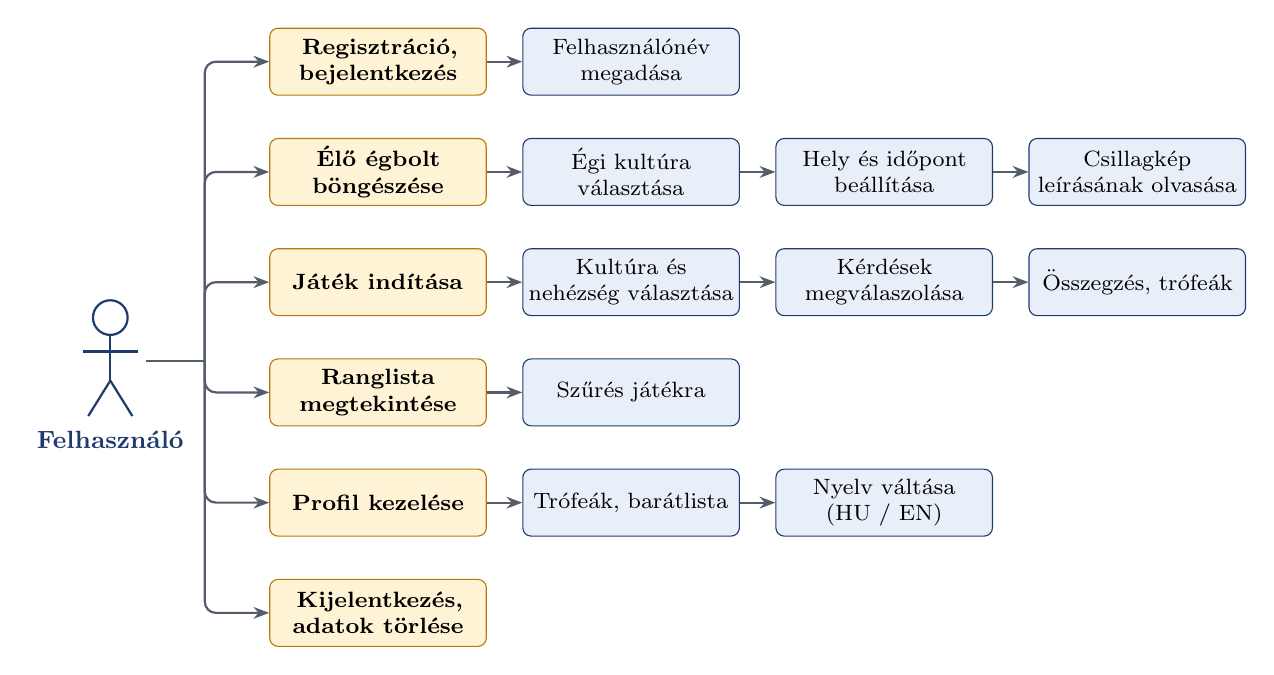
\begin{tikzpicture}[
      eset/.style={rectangle,rounded corners=3pt,draw=egkek,fill=egkekvil,
                   minimum width=2.75cm,minimum height=0.85cm,align=center,
                   font=\footnotesize,inner sep=2pt,text width=2.6cm},
      fo/.style={eset,fill=aranyvil,draw=arany,font=\footnotesize\bfseries},
      nyil/.style={-{Stealth[length=2mm]},thick,draw=szurke},
      ag/.style={thick,draw=szurke,rounded corners=4pt}]
    \palcika{0,-3.4}{fh}{Felhasználó}

    % Fő funkciók (sorok) és lépéseik
    \node[fo] (r1) at (3.4, 0.4)  {Regisztráció, bejelentkezés};
    \node[eset,right=0.45cm of r1] (r1b) {Felhasználónév megadása};

    \node[fo] (r2) at (3.4,-1.0)  {Élő égbolt böngészése};
    \node[eset,right=0.45cm of r2] (r2b) {Égi kultúra választása};
    \node[eset,right=0.45cm of r2b] (r2c) {Hely és időpont beállítása};
    \node[eset,right=0.45cm of r2c] (r2d) {Csillagkép leírásának olvasása};

    \node[fo] (r3) at (3.4,-2.4)  {Játék indítása};
    \node[eset,right=0.45cm of r3] (r3b) {Kultúra és nehézség választása};
    \node[eset,right=0.45cm of r3b] (r3c) {Kérdések megválaszolása};
    \node[eset,right=0.45cm of r3c] (r3d) {Összegzés, trófeák};

    \node[fo] (r4) at (3.4,-3.8)  {Ranglista megtekintése};
    \node[eset,right=0.45cm of r4] (r4b) {Szűrés játékra};

    \node[fo] (r5) at (3.4,-5.2)  {Profil kezelése};
    \node[eset,right=0.45cm of r5] (r5b) {Trófeák, barátlista};
    \node[eset,right=0.45cm of r5b] (r5c) {Nyelv váltása (HU / EN)};

    \node[fo] (r6) at (3.4,-6.6)  {Kijelentkezés, adatok törlése};

    % Elágazás a szereplőtől
    \coordinate (bus) at (1.2,-3.4);
    \draw[thick,szurke] (0.45,-3.4) -- (bus);
    \foreach \r in {r1,r2,r3,r4,r5,r6}
      \draw[nyil,rounded corners=4pt] (bus) |- (\r.west);

    \foreach \a/\b in {r1/r1b,r2/r2b,r2b/r2c,r2c/r2d,r3/r3b,r3b/r3c,r3c/r3d,r4/r4b,r5/r5b,r5b/r5c}
      \draw[nyil] (\a) -- (\b);
  \end{tikzpicture}
  \caption{Esetdiagram}
  \label{fig:eset}
\end{figure}

A felhasználói interakciókat az \ref{fig:eset}.~ábra szemlélteti. A rendszer elsődleges
szereplője a \textbf{Felhasználó}. Bejelentkezés nélkül csak a kezdőképernyő, a regisztráció és
a nyelvválasztás érhető el; bejelentkezés után a következő funkciók használhatók:

\textbf{Regisztráció, bejelentkezés:} a felhasználó e-mail-címmel és jelszóval hoz létre fiókot,
majd egyedi felhasználónevet választ, amely a ranglistán és a barátoknál megjelenik.

\textbf{Élő égbolt böngészése:} a központi funkció. A felhasználó húzással forgatja, görgővel vagy
két ujjal nagyítja az eget, kiválasztja az égi kultúrát, a megfigyelés helyét és időpontját, és egy
csillagképre koppintva elolvassa a hozzá tartozó leírást.

\textbf{Játék indítása:} három játék közül választhat (Csillagkép-felismerő, Csillagról
csillagra, Hiedelem-találó). Indítás előtt kiválasztja az égi kultúrát és a nehézséget, a
játék végén összegzést és az esetleg megszerzett trófeákat látja.

\textbf{Ranglista megtekintése:} az összesített vagy játékonkénti legjobb eredmények listája,
a saját helyezés kiemelésével.

\textbf{Profil kezelése:} a megszerzett trófeák, a barátlista, a nyelv beállítása.

\textbf{Kijelentkezés, adatok törlése:} a munkamenet lezárása, illetve a fiók és minden
hozzá tartozó adat végleges törlése (jelszavas megerősítéssel).

\subsection{Rendszerkövetelmények}

A projekt célja egy webes és mobilos (Android, iOS) felületen egyaránt futó, csillagászati és
kulturális ismeretterjesztő alkalmazás elkészítése. A rendszer alapját a TypeScript nyelv, a
React Native és az Expo keretrendszer képezi; a háromdimenziós égboltot a three.js grafikus
könyvtár rajzolja WebGL-en keresztül. A csillagkatalógus (8943 csillag) és a 18 égi kultúra
(összesen 375 alakzat) adatai az alkalmazásba csomagolt JSON-fájlokban vannak, így az égbolt
böngészése internetkapcsolat nélkül is működik. A felhasználói fiókok, a játékeredmények, a
ranglista és a barátlista a Firebase felhőszolgáltatásban (Authentication, Cloud Firestore)
tárolódnak. Fejlesztéshez és bemutatáshoz az alkalmazás Firebase nélkül, úgynevezett
\emph{helyi módban} is elindul: ilyenkor a fiókok és az eredmények a készüléken maradnak.

\subsubsection{Funkcionális követelmények}

A következő táblázat összefoglalja a \textbf{Csillagnéző} által biztosított funkciókat, a
belépéstől az égbolt böngészésén és a játékokon át a ranglistáig és a profilig.

{\small
\begin{longtable}{|L{4.3cm}|L{10.75cm}|}
  \caption{Funkcionális követelmények}\label{tab:funkc}\\
  \hline
  \fejlec\textbf{Funkció} & \textbf{Leírás} \\ \hline
  \endfirsthead
  \hline
  \fejlec\textbf{Funkció} & \textbf{Leírás} \\ \hline
  \endhead
  Regisztráció és bejelentkezés & E-mail-cím és legalább 6 karakteres jelszó megadásával. A
  hibás vagy foglalt adatokra az űrlap érthető, lefordított hibaüzenettel válaszol. \\ \hline
  Felhasználónév & 3-24 karakteres, csak betűt, számot, aláhúzást és kötőjelet tartalmazó,
  egyedi név. A foglalás tranzakcióban történik, így két felhasználó nem kaphatja meg ugyanazt a
  nevet. \\ \hline
  Élő égbolt & A szabad szemmel látható csillagok (6,5 magnitúdóig), valamint minden, valamelyik
  csillagképben szereplő csillag megjelenítése. A pontméret a fényességtől, a szín a csillag
  színindexétől függ. \\ \hline
  Navigáció az égen & Húzással forgatás, görgővel vagy két ujjal nagyítás (15°-100°-os
  látómező), egy gombnyomással visszatérés az alapnézetbe (észak felé, 35°-os magasságban). \\ \hline
  Égi kultúra választása & 18 kultúra kereshető listából (pl. magyar népi, nyugati, román,
  skandináv, hawaii, maori). A választás azonnal frissíti a vonalakat és a neveket. \\ \hline
  Csillagképvonalak, nevek, föld & A vonalak, a csillagképnevek és a földfelszín (horizont alatti
  föld, horizont menti derengés) külön-külön ki- és bekapcsolható. A nevek nem takarják egymást,
  az égtájakat betűk jelzik. \\ \hline
  Csillagkép-leírás & Egy csillagképre koppintva kiemelődik az alakzat, és megnyílik a leírás:
  eredeti név, legenda, hiedelem, a csillagok száma. \\ \hline
  Megfigyelési hely & A készülék helymeghatározása (engedély esetén) vagy 22 előre megadott város
  közül választás. \\ \hline
  Időutazás & Az időpont tetszőleges beállítása i.\,e.\ 1001 és i.\,sz.\ 3000 között
  (évcsúszka, napon belüli idő, ±1 nap / ±1 év lépés), visszatérés a jelenbe egy gombbal. \\ \hline
  Játékok & Csillagkép-felismerő (10 kör), Csillagról csillagra (5 kör), Hiedelem-találó (8
  kör). Mindegyikben választható kultúra és nehézség; nehéz fokozatban dupla pont jár. \\ \hline
  Pontszámítás & Helyes válaszért alappont, gyorsasági és sorozatbónusz; az összekötős játékban
  vonalanként pont, hibáért és segítségért levonás. \\ \hline
  Eredmények mentése & Játékonként a legjobb pontszám a készüléken és a felhőben is mentődik;
  hálózati hiba esetén az eredmény sorba áll, és később automatikusan elküldődik. \\ \hline
  Trófeák & 12 trófea (pl. Első fény, Hibátlan, Csillagász) automatikus kiosztása a
  játékstatisztika alapján; a játék végén „Új trófea” jelzés. \\ \hline
  Ranglista & Összesített és játékonkénti toplista (legfeljebb 50 játékos), élő frissítéssel. A
  saját helyezés akkor is látszik, ha a felhasználó nincs a toplistában. \\ \hline
  Barátlista & Barátkód alapján legfeljebb 50 barát felvétele; a barátok neve, összpontja és
  trófeáinak száma látszik. \\ \hline
  Nyelvváltás & A teljes felület és a csillagképek leírásai magyarul és angolul, újraindítás
  nélküli váltással; a választás megmarad. \\ \hline
  Fiók törlése & A fiók, a profil, a ranglista-bejegyzés és a barátlista végleges törlése
  jelszavas megerősítés után. \\ \hline
\end{longtable}
}

\subsubsection{Nem funkcionális követelmények}

Ez a szakasz a rendszer minőségi jellemzőit és működési peremfeltételeit rögzíti, amelyek nem
közvetlenül a funkciókra, hanem a felhasználói élményre, a megbízhatóságra, a biztonságra és a
karbantarthatóságra vonatkoznak.

{\small
\begin{longtable}{|L{4.3cm}|L{10.75cm}|}
  \caption{Nem funkcionális követelmények}\label{tab:nemfunkc}\\
  \hline
  \fejlec\textbf{Típus} & \textbf{Leírás} \\ \hline
  \endfirsthead
  \hline
  \fejlec\textbf{Típus} & \textbf{Leírás} \\ \hline
  \endhead
  Teljesítmény & A csillagok egyetlen pontfelhőként, egy rajzolási hívással kerülnek a
  képernyőre; a jelenet csak változáskor rajzolódik újra. Az égbolt telefonon is akadásmentesen
  forgatható. \\ \hline
  Hordozhatóság & Egyetlen kódbázis web, Android (7-es verziótól) és iOS (16.4-es verziótól)
  platformra. \\ \hline
  Megbízhatóság & Az égbolt internet nélkül is működik; az eredmények hálózati hiba esetén
  sorba állnak. A Firestore-ból érkező adatokat a kliens ellenőrzi, mielőtt felhasználná. \\ \hline
  Biztonság & A Firestore biztonsági szabályai szerint mindenki csak a saját dokumentumait
  írhatja; a nyilvános ranglistába nem kerül e-mail-cím. A naplóban a jelszavak, tokenek helyett
  \kod{[REDACTED]} áll, az e-mail-címek maszkolva jelennek meg. \\ \hline
  Használhatóság & Reszponzív elrendezés három képernyőméretre (telefon, tablet, asztali); telefonon
  alsó ikonsáv és ujjal lapozható oldalak. Billentyűzetes fókuszjelzés, a csökkentett mozgás
  rendszerbeállítás tiszteletben tartása. \\ \hline
  Lokalizáció & Magyar és angol felület, típusosan ellenőrzött fordítási kulcsokkal; új nyelv
  egy szótárfájllal felvehető. \\ \hline
  Skálázhatóság (tartalom) & Új égi kultúra egy JSON-fájllal (és angol fordításával), új játék
  néhány jól körülhatárolt ponton vehető fel. \\ \hline
  Karbantarthatóság & Szigorú TypeScript-típusellenőrzés, ESLint és Prettier, 361 automatikus
  egységteszt. \\ \hline
  Jogi megfelelés & A csillag- és kultúraadatok nyílt licencűek (CC BY-SA, CC BY), a forrásokat
  az \kod{ATTRIBUTION.md} fájl sorolja fel. \\ \hline
\end{longtable}
}

\subsubsection{Technológiai specifikáció}

A technológiai specifikáció a fejlesztéshez és a futtatáshoz szükséges szoftveres környezetet
rögzíti. Az alkalmazás logikája és megjelenítése TypeScript nyelven, a React Native és Expo
keretrendszerre épül; a háromdimenziós égboltot a three.js és a React Three Fiber rajzolja. A
felhasználói adatok tárolását a Firebase felhőszolgáltatás végzi, a helyi adatokat pedig a
készülék kulcs-érték tárolója.

{\small
\begin{longtable}{|L{4.3cm}|L{10.75cm}|}
  \caption{Felhasznált technológiák}\label{tab:tech}\\
  \hline
  \fejlec\textbf{Technológia} & \textbf{Részletek} \\ \hline
  \endfirsthead
  \hline
  \fejlec\textbf{Technológia} & \textbf{Részletek} \\ \hline
  \endhead
  TypeScript 6 & A teljes alkalmazás nyelve, szigorú típusellenőrzéssel. \\ \hline
  React 19 és React Native 0.88 & A felhasználói felület komponensalapú felépítése; a webes
  változathoz a React Native for Web. \\ \hline
  Expo SDK 58, Expo Router & Fejlesztői környezet, natív modulok (GL, helymeghatározás,
  fájlrendszer), fájlalapú útvonalkezelés. \\ \hline
  three.js és React Three Fiber & A 3D égbolt (csillagok, vonalak, föld) WebGL-alapú
  megjelenítése; saját GLSL árnyaló a csillagokhoz. \\ \hline
  Zustand & Könnyűsúlyú állapotkezelés (égbolt-beállítások, nézet, bejelentkezés). \\ \hline
  Firebase 12 & Authentication (e-mail és jelszó), Cloud Firestore (profil, ranglista,
  barátlista, felhasználónevek), helyi emulátor a teszteléshez. \\ \hline
  AsyncStorage & Helyi kulcs-érték tároló (weben a böngésző \kod{localStorage}-a): nyelv,
  helyi fiókok, eredménysor, statisztika. \\ \hline
  Jest, ESLint, Prettier & Egységtesztek, statikus kódelemzés, egységes kódformázás. \\ \hline
  Python 3 szkriptek & A csillagkatalógus (HYG adatbázis) és a nyugati égi kultúra (Stellarium)
  adatainak előállítása. \\ \hline
  Git és GitHub & Verziókezelés, feature branch-ek, pull requestek, kódáttekintés. \\ \hline
\end{longtable}
}

% =====================================================================
\section{Tervezés}

\begin{figure}[H]
  \centering
  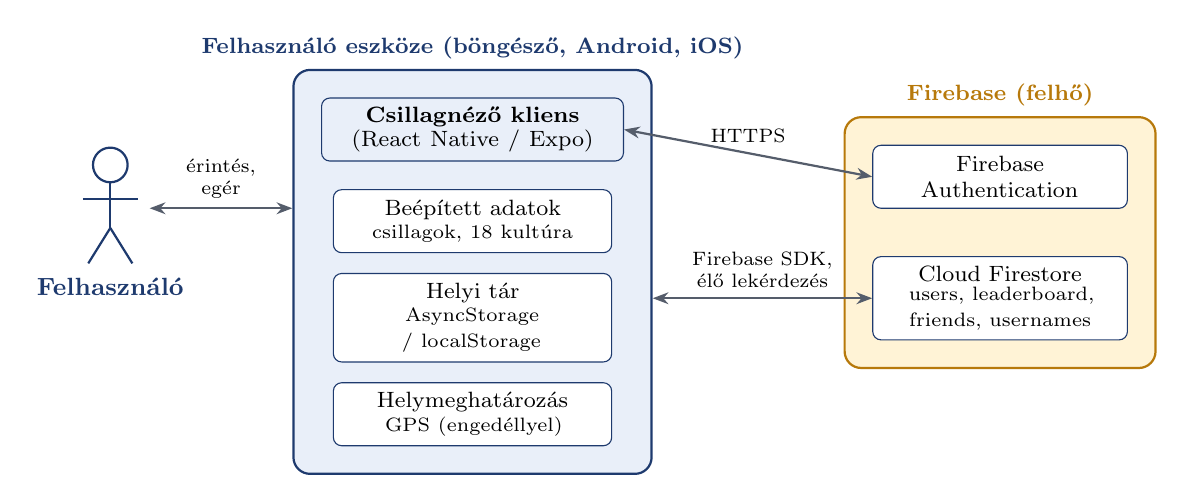
\begin{tikzpicture}[
      doboz/.style={rectangle,rounded corners=3pt,draw=egkek,fill=white,align=center,
                    font=\footnotesize,minimum height=0.8cm,text width=3.3cm},
      kulso/.style={rectangle,rounded corners=6pt,draw=egkek,thick,fill=egkekvil},
      felho/.style={rectangle,rounded corners=6pt,draw=arany,thick,fill=aranyvil},
      kapcs/.style={{Stealth[length=2mm]}-{Stealth[length=2mm]},thick,draw=szurke}]
    \palcika{0,0}{fh}{Felhasználó}

    \node[doboz,fill=egkekvil,font=\footnotesize\bfseries,text width=3.6cm] (kliens) at (4.6,1.0)
      {Csillagnéző kliens\\[-1pt]{\normalfont (React Native / Expo)}};
    \node[doboz,below=0.35cm of kliens] (adat) {Beépített adatok\\[-1pt]{\scriptsize csillagok, 18 kultúra}};
    \node[doboz,below=0.25cm of adat] (helyi) {Helyi tár\\[-1pt]{\scriptsize AsyncStorage / localStorage}};
    \node[doboz,below=0.25cm of helyi] (gps) {Helymeghatározás\\[-1pt]{\scriptsize GPS (engedéllyel)}};
    \begin{scope}[on background layer]
      \node[kulso,fit=(kliens)(gps),inner sep=0.35cm,label={[font=\footnotesize\bfseries,text=egkek]above:Felhasználó eszköze (böngésző, Android, iOS)}] (eszkoz) {};
    \end{scope}

    \node[doboz,text width=3cm] (auth) at (11.3,0.4) {Firebase\\ Authentication};
    \node[doboz,text width=3cm,below=0.6cm of auth] (fs) {Cloud Firestore\\[-1pt]{\scriptsize users, leaderboard,\\ friends, usernames}};
    \begin{scope}[on background layer]
      \node[felho,fit=(auth)(fs),inner sep=0.35cm,label={[font=\footnotesize\bfseries,text=arany]above:Firebase (felhő)}] (firebase) {};
    \end{scope}

    \draw[kapcs] (0.5,0) -- node[above,font=\scriptsize,align=center]{érintés,\\ egér} (eszkoz.west |- fh);
    \draw[kapcs] (kliens.east) -- node[above,font=\scriptsize]{HTTPS} (auth.west);
    \draw[kapcs] (eszkoz.east |- fs.west) -- node[above,font=\scriptsize,align=center]{Firebase SDK,\\ élő lekérdezés} (fs.west);
  \end{tikzpicture}
  \caption{A rendszer fizikai felépítése}
  \label{fig:telepites}
\end{figure}

\subsection{Architektúra}

Az alkalmazás háromrétegű architektúrára épül, amely jól elválasztja a megjelenítést, az
alkalmazás logikáját és az adatok kezelését. A \ref{fig:telepites}.~ábra a rendszer fizikai
felépítését szemlélteti:

\textbf{Interakció (Felhasználó - eszköz):} a felhasználó böngészőben vagy telefonon, érintéssel,
egérrel, görgővel és billentyűzettel kezeli az alkalmazást.

\textbf{Feldolgozás (kliens):} a teljes alkalmazáslogika - a csillagászati számítások, a
játékok, a pontszámítás - a felhasználó eszközén fut. Az égbolt adatai az alkalmazásba vannak
csomagolva, ezért az égbolt böngészéséhez nincs szükség hálózatra.

\textbf{Adattárolás (helyi tár és felhő):} a beállítások és a helyi eredmények a készülék
kulcs-érték tárolójába kerülnek. A fiókokat a Firebase Authentication, a profilokat, a
ranglistát és a barátlistát a Cloud Firestore kezeli; a ranglista élő lekérdezéssel
(\emph{snapshot listener}) azonnal frissül, ha bárki új eredményt ér el.

A kód rétegeit és fő moduljait a \ref{fig:retegek}.~ábra mutatja.

\begin{figure}[H]
  \centering
  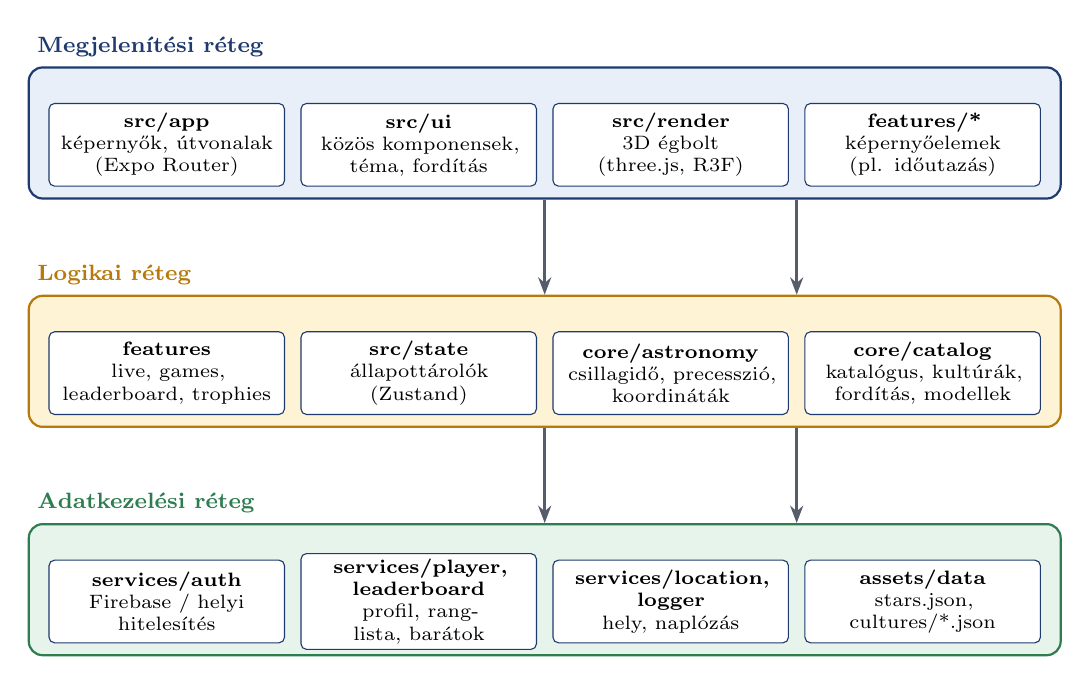
\begin{tikzpicture}[
      modul/.style={rectangle,rounded corners=2pt,draw=egkek,fill=white,align=center,
                    font=\scriptsize,minimum height=1.05cm,text width=2.85cm,inner sep=2pt},
      reteg/.style={rectangle,rounded corners=5pt,draw=#1,thick,inner sep=0.25cm},
      cim/.style={font=\footnotesize\bfseries,anchor=south west},
      le/.style={-{Stealth[length=2.2mm]},very thick,draw=szurke}]
    % Megjelenítési réteg
    \node[modul] (app)    at (0,0)    {\textbf{src/app}\\ képernyők, útvonalak\\ (Expo Router)};
    \node[modul] (ui)     at (3.2,0)  {\textbf{src/ui}\\ közös komponensek,\\ téma, fordítás};
    \node[modul] (render) at (6.4,0)  {\textbf{src/render}\\ 3D égbolt\\ (three.js, R3F)};
    \node[modul] (feat1)  at (9.6,0)  {\textbf{features/*}\\ képernyőelemek\\ (pl. időutazás)};
    \begin{scope}[on background layer]
      \node[reteg=egkek,fill=egkekvil,fit=(app)(feat1),inner ysep=0.3cm,yshift=0.15cm] (r1) {};
    \end{scope}
    \node[cim,text=egkek] at (r1.north west) {Megjelenítési réteg};

    % Logikai réteg
    \node[modul] (live)   at (0,-2.9)   {\textbf{features}\\ live, games,\\ leaderboard, trophies};
    \node[modul] (state)  at (3.2,-2.9) {\textbf{src/state}\\ állapottárolók\\ (Zustand)};
    \node[modul] (astro)  at (6.4,-2.9) {\textbf{core/astronomy}\\ csillagidő, precesszió,\\ koordináták};
    \node[modul] (cat)    at (9.6,-2.9) {\textbf{core/catalog}\\ katalógus, kultúrák,\\ fordítás, modellek};
    \begin{scope}[on background layer]
      \node[reteg=arany,fill=aranyvil,fit=(live)(cat),inner ysep=0.3cm,yshift=0.15cm] (r2) {};
    \end{scope}
    \node[cim,text=arany] at (r2.north west) {Logikai réteg};

    % Adatkezelési réteg
    \node[modul] (auth)   at (0,-5.8)   {\textbf{services/auth}\\ Firebase / helyi\\ hitelesítés};
    \node[modul] (player) at (3.2,-5.8) {\textbf{services/player,}\\ \textbf{leaderboard}\\ profil, ranglista, barátok};
    \node[modul] (other)  at (6.4,-5.8) {\textbf{services/location,}\\ \textbf{logger}\\ hely, naplózás};
    \node[modul] (assets) at (9.6,-5.8) {\textbf{assets/data}\\ stars.json,\\ cultures/*.json};
    \begin{scope}[on background layer]
      \node[reteg=zold,fill=zoldvil,fit=(auth)(assets),inner ysep=0.3cm,yshift=0.15cm] (r3) {};
    \end{scope}
    \node[cim,text=zold] at (r3.north west) {Adatkezelési réteg};

    \foreach \x in {4.8,8.0}{
      \draw[le] (\x,0 |- r1.south) -- (\x,0 |- r2.north);
      \draw[le] (\x,0 |- r2.south) -- (\x,0 |- r3.north);
    }
  \end{tikzpicture}
  \caption{A kód rétegei és fő moduljai}
  \label{fig:retegek}
\end{figure}

\subsubsection{Megjelenítési réteg}

A felhasználóval való interakcióért felelős. Ide tartoznak az Expo Router által kezelt képernyők
(bejelentkezés, élő égbolt, játékok, ranglista, profil, a teljes képernyős játékok), a közös
felületi elemek (gombok, kártyák, legördülő listák, lapok, az alsó és oldalsó menüsáv), a téma
(színek, térközök, betűméretek) és a fordítás. A 3D égboltot a \kod{src/render} modul rajzolja: a
csillagokat egyetlen pontfelhőként, saját GLSL árnyalóval, a csillagképvonalakat
szakaszlistaként, a földet félgömbként. A csillagképnevek és az égtájbetűk a 3D jelenet fölötti,
képernyő-koordinátás rétegben jelennek meg, egymást nem takarva.

\subsubsection{Logikai réteg}

Az alkalmazás működési szabályai itt valósulnak meg. Kezeli:

\begin{itemize}
  \item a csillagászati számításokat: Julián-dátum, greenwichi és helyi csillagidő, az IAU 2006
        precessziós modell, az egyenlítői és horizontális koordináták közötti átváltás;
  \item az égi kultúrák és a csillagkatalógus betöltését, a nyelv szerinti fordítását;
  \item az égbolt és a nézet állapotát (kultúra, hely, időpont, kamera iránya, látómező);
  \item a játékok logikáját (kérdések sorsolása, válaszok kiértékelése, pontszámítás);
  \item a trófeák feltételeinek kiértékelését és a ranglista rangsorolását.
\end{itemize}

A logikai réteg tiszta, platformfüggetlen TypeScript-függvényekből áll, ezért jól tesztelhető;
a megjelenítési és az adatkezelési réteg között interfészeket biztosít.

\subsubsection{Adatkezelési réteg}

A perzisztens adatok tárolásáért felelős. A szolgáltatások közös interfész mögött két
megvalósítással rendelkeznek: Firebase-alapúval (éles használatra) és helyivel (Firebase
nélküli fejlesztéshez, bemutatáshoz). Így például a \kod{LeaderboardService} interfészt a
\kod{FirebaseLeaderboardService} és a \kod{LocalLeaderboardService} is megvalósítja, a felület
pedig nem tudja, és nem is kell tudnia, melyikkel dolgozik. Ide tartozik a helymeghatározás és a
központi naplózás is, amely a bizalmas adatokat (jelszavak, tokenek, e-mail-címek) kiszűri.

\subsection{Modulok leírása}

Az egyes rétegek közötti kommunikáció meghatározott adatfolyamon keresztül történik. A
megjelenítési réteg feldolgozza a felhasználói műveleteket (koppintás, húzás, gombnyomás), és
továbbadja őket a logikai rétegnek, amely eldönti, hogyan reagáljon az alkalmazás (például új
időpont, új kérdés, válasz kiértékelése). Ha adat szükséges, a logikai réteg az adatkezelési
réteghez fordul, amely visszaadja a kért adatokat (például a ranglistát), vagy elmenti az újakat
(például egy játék eredményét). Végül a megjelenítés frissül, és a felhasználó látja az
eredményt. Az alábbiakban a három legfontosabb modult mutatjuk be részletesebben.

\subsubsection*{Az égbolt kiszámítása és kirajzolása}

A csillagkatalógus a csillagok J2000.0 epochára vonatkozó egyenlítői koordinátáit (rektaszcenzió,
deklináció), fényességét és színindexét tartalmazza. A csillagonkénti számítás elkerülésére a
teljes égboltgömböt egyetlen forgatási mátrixszal helyezzük a megfigyelő horizontjába:
\[
  M = W \cdot R_z(-\mathrm{LST}) \cdot P ,
\]
ahol $P$ az IAU 2006 precessziós mátrix (J2000-ről a megadott dátumra), $R_z(-\mathrm{LST})$ a
helyi csillagidő szerinti forgatás, $W$ pedig a földrajzi szélességtől függő átváltás a
horizontális rendszerbe. A mátrixot csak az időpont vagy a hely változásakor kell újraszámolni; a
csillagok, a vonalak és a nevek ugyanazt a mátrixot használják (\ref{fig:egbolt}.~ábra). A
számítások helyességét az egységtesztek egy független csillagászati könyvtár (astronomy-engine)
eredményeivel vetik össze.

\begin{figure}[H]
  \centering
  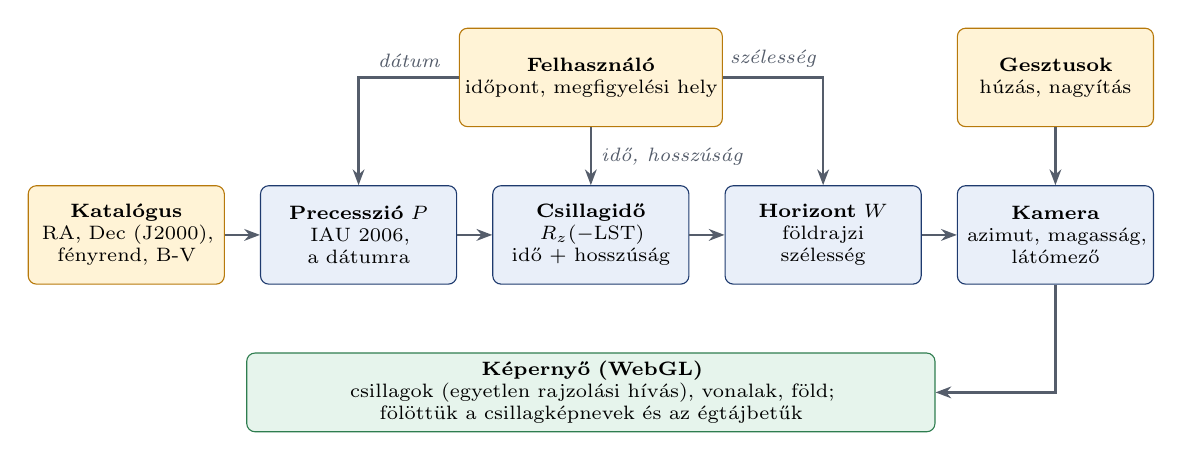
\begin{tikzpicture}[
      lepes/.style={rectangle,rounded corners=3pt,draw=egkek,fill=egkekvil,align=center,
                    font=\scriptsize,minimum height=1.25cm,text width=2.35cm,inner sep=2pt},
      be/.style={lepes,fill=aranyvil,draw=arany},
      nyil/.style={-{Stealth[length=2mm]},thick,draw=szurke}]
    \node[be]    (k) at (0,0)     {\textbf{Katalógus}\\ RA, Dec (J2000),\\ fényrend, B-V};
    \node[lepes] (p) at (2.95,0)  {\textbf{Precesszió} $P$\\ IAU 2006,\\ a dátumra};
    \node[lepes] (s) at (5.9,0)   {\textbf{Csillagidő}\\ $R_z(-\mathrm{LST})$\\ idő + hosszúság};
    \node[lepes] (w) at (8.85,0)  {\textbf{Horizont} $W$\\ földrajzi\\ szélesség};
    \node[lepes] (c) at (11.8,0)  {\textbf{Kamera}\\ azimut, magasság,\\ látómező};
    \node[be,text width=3.2cm] (i) at (5.9,2.0) {\textbf{Felhasználó}\\ időpont, megfigyelési hely};
    \node[be]    (g) at (11.8,2.0) {\textbf{Gesztusok}\\ húzás, nagyítás};
    \node[lepes,text width=8.6cm,fill=zoldvil,draw=zold,minimum height=1.0cm] (out) at (5.9,-2.0)
      {\textbf{Képernyő (WebGL)}\\ csillagok (egyetlen rajzolási hívás), vonalak, föld;\\ fölöttük a csillagképnevek és az égtájbetűk};
    \draw[nyil] (k) -- (p); \draw[nyil] (p) -- (s); \draw[nyil] (s) -- (w); \draw[nyil] (w) -- (c);
    \draw[nyil] (i.west) -| node[pos=0.25,above,font=\scriptsize\itshape,text=szurke]{dátum} (p.north);
    \draw[nyil] (i.south) -- node[right,font=\scriptsize\itshape,text=szurke]{idő, hosszúság} (s.north);
    \draw[nyil] (i.east) -| node[pos=0.25,above,font=\scriptsize\itshape,text=szurke]{szélesség} (w.north);
    \draw[nyil] (g) -- (c);
    \draw[nyil] (c.south) |- (out.east);
  \end{tikzpicture}
  \caption{Az égbolt kiszámításának és kirajzolásának folyamata}
  \label{fig:egbolt}
\end{figure}

A koppintás kiértékelése (melyik csillagképre koppintott a felhasználó) ugyanezzel a vetítéssel,
a képernyőre vetített vonalaktól és nevektől mért távolság alapján történik, így ujjal is könnyű
eltalálni egy alakzatot. Húzás és nagyítás közben a nézet legfeljebb képkockánként frissül, ezért
a mozgatás telefonon is gördülékeny.

\subsubsection*{Játékok és eredménykezelés}

A három játék közös keretben fut: indítás előtt a felhasználó kultúrát és nehézséget választ, a
játék végén összegzést kap. A \ref{fig:szekvencia}.~ábra egy játék időbeli lefolyását mutatja
a kérdéstől az eredmény felhőbe mentéséig.

\begin{figure}[htbp]
  \centering
  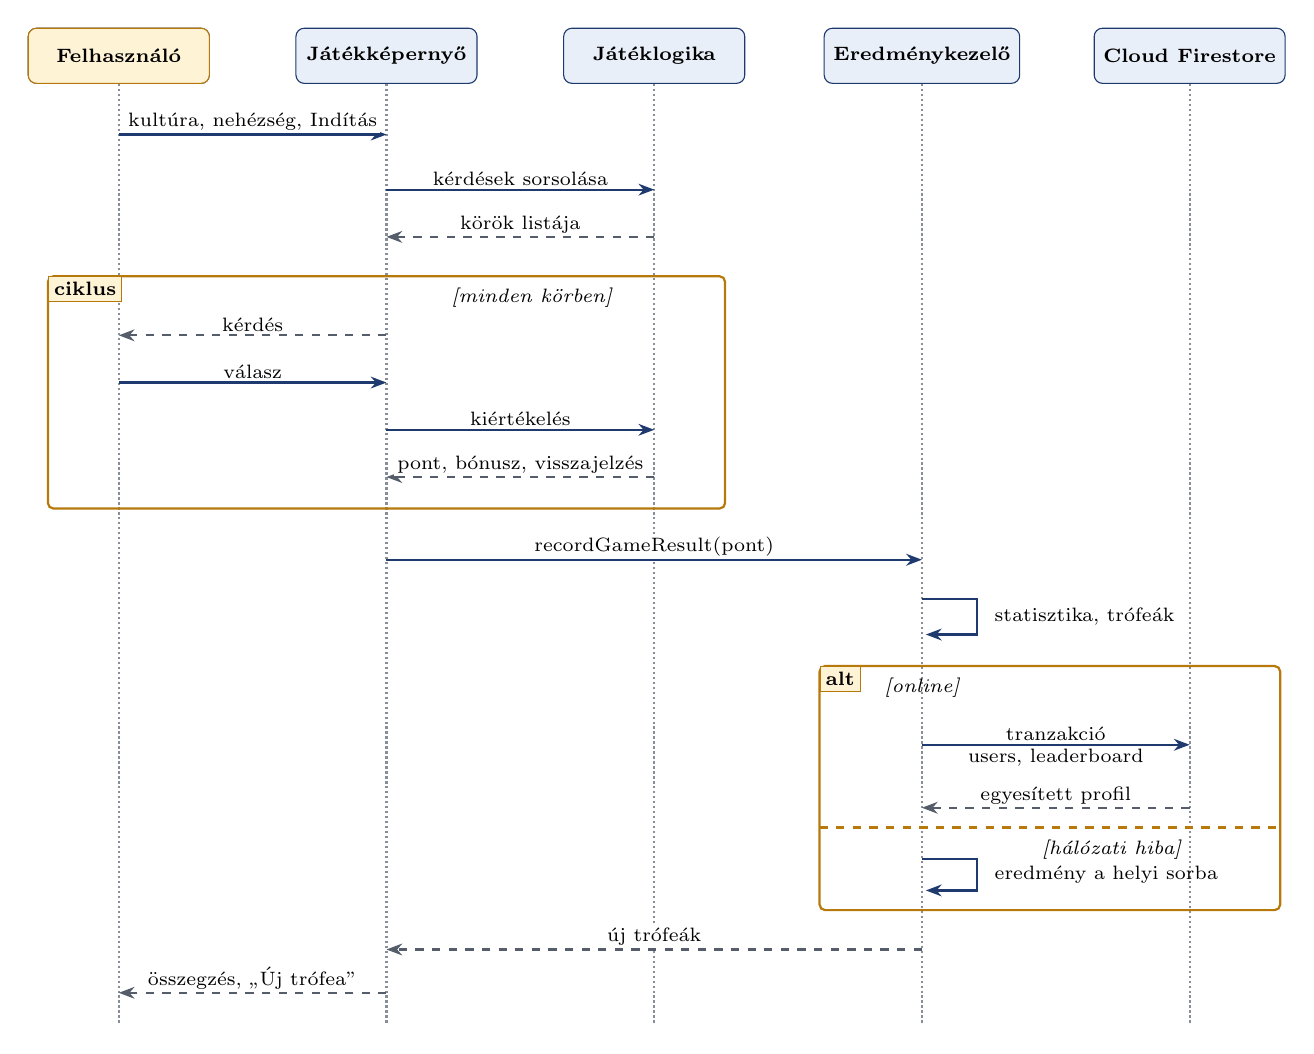
\begin{tikzpicture}[
      resztv/.style={rectangle,rounded corners=3pt,draw=egkek,fill=egkekvil,font=\scriptsize\bfseries,
                     minimum width=2.3cm,minimum height=0.7cm,align=center},
      elet/.style={densely dotted,thick,draw=szurke!70},
      hiv/.style={-{Stealth[length=2mm]},thick,draw=egkek},
      vissza/.style={-{Stealth[length=2mm]},thick,dashed,draw=szurke},
      uz/.style={font=\scriptsize,fill=white,inner sep=1pt},
      keret/.style={draw=arany,thick,rounded corners=2pt},
      kcimke/.style={font=\scriptsize\bfseries,fill=aranyvil,draw=arany,inner sep=2pt,anchor=north west}]
    % Résztvevők
    \foreach \x/\n/\t in {0/u/Felhasználó,3.4/ui/Játékképernyő,6.8/gl/Játéklogika,10.2/res/Eredménykezelő,13.6/fs/Cloud Firestore}{
      \node[resztv] (\n) at (\x,0) {\t};
      \draw[elet] (\n.south) -- (\x,-12.3);
    }
    \node[resztv,fill=aranyvil,draw=arany] at (0,0) {Felhasználó};
    % Indítás
    \draw[hiv] (0,-1.0) -- node[uz,above]{kultúra, nehézség, Indítás} (3.4,-1.0);
    \draw[hiv] (3.4,-1.7) -- node[uz,above]{kérdések sorsolása} (6.8,-1.7);
    \draw[vissza] (6.8,-2.3) -- node[uz,above]{körök listája} (3.4,-2.3);
    % Ciklus
    \draw[keret] (-0.9,-2.8) rectangle (7.7,-5.75);
    \node[kcimke] at (-0.9,-2.8) {ciklus};
    \node[font=\scriptsize\itshape,anchor=north west] at (4.1,-2.83) {[minden körben]};
    \draw[vissza] (3.4,-3.55) -- node[uz,above]{kérdés} (0,-3.55);
    \draw[hiv] (0,-4.15) -- node[uz,above]{válasz} (3.4,-4.15);
    \draw[hiv] (3.4,-4.75) -- node[uz,above]{kiértékelés} (6.8,-4.75);
    \draw[vissza] (6.8,-5.35) -- node[uz,above]{pont, bónusz, visszajelzés} (3.4,-5.35);
    % Eredmény
    \draw[hiv] (3.4,-6.4) -- node[uz,above]{recordGameResult(pont)} (10.2,-6.4);
    \draw[hiv] (10.2,-6.9) -- (10.9,-6.9) -- (10.9,-7.35) -- (10.25,-7.35);
    \node[font=\scriptsize,anchor=west] at (11.0,-7.12) {statisztika, trófeák};
    % Alt
    \draw[keret] (8.9,-7.75) rectangle (14.75,-10.85);
    \node[kcimke] at (8.9,-7.75) {alt};
    \node[font=\scriptsize\itshape,anchor=north west] at (9.6,-7.78) {[online]};
    \draw[hiv] (10.2,-8.75) -- node[uz,above]{tranzakció} node[uz,below]{users, leaderboard} (13.6,-8.75);
    \draw[vissza] (13.6,-9.55) -- node[uz,above]{egyesített profil} (10.2,-9.55);
    \draw[keret,dashed] (8.9,-9.8) -- (14.75,-9.8);
    \node[font=\scriptsize\itshape,anchor=north west] at (11.6,-9.83) {[hálózati hiba]};
    \draw[hiv] (10.2,-10.2) -- (10.9,-10.2) -- (10.9,-10.6) -- (10.25,-10.6);
    \node[font=\scriptsize,anchor=west] at (11.0,-10.4) {eredmény a helyi sorba};
    % Vége
    \draw[vissza] (10.2,-11.35) -- node[uz,above]{új trófeák} (3.4,-11.35);
    \draw[vissza] (3.4,-11.9) -- node[uz,above]{összegzés, „Új trófea”} (0,-11.9);
  \end{tikzpicture}
  \caption{Egy játék lefolyása (szekvenciadiagram)}
  \label{fig:szekvencia}
\end{figure}

\begin{itemize}
  \item A felhasználó kiválasztja a kultúrát és a nehézséget, majd elindítja a játékot.
  \item A játéklogika kisorsolja a köröket a kiválasztott kultúra csillagképeiből (a
        Hiedelem-találónál csak azokból, amelyekhez elég hosszú leírás tartozik).
  \item Minden körben a felhasználó válaszol, a logika kiértékeli a választ:
        \begin{itemize}
          \item helyes válasznál alappontot, gyorsasági és sorozatbónuszt ad;
          \item helytelen válasznál nem jár pont, a sorozat megszakad, és az alkalmazás megmutatja
                a helyes választ.
        \end{itemize}
  \item A játék végén az eredménykezelő frissíti a helyi statisztikát, kiértékeli a trófeákat,
        majd egyetlen Firestore-tranzakcióban frissíti a felhasználó profilját és nyilvános
        ranglista-bejegyzését. Hálózati hiba esetén az eredmény a helyi sorba kerül, és a
        következő alkalommal automatikusan elküldődik.
  \item A ranglistát figyelő képernyők az élő lekérdezésen keresztül azonnal megkapják az új
        eredményt.
\end{itemize}

\subsubsection*{Adatmodell}

Az adatok két csoportba sorolhatók (\ref{fig:adatmodell}.~ábra). A \textbf{statikus adatok} az
alkalmazásba vannak csomagolva, és csak olvashatók: a csillagkatalógus és az égi kultúrák. A
csillagképek vonalait a csillagok Hipparcos-azonosítói (HIP) írják le, így egy kultúra
alakzatai a katalógus csillagaira hivatkoznak. Minden kultúrához angol fordításfájl tartozik,
amely felülírja a magyar neveket és leírásokat, ha angol a felület nyelve. A
\textbf{felhasználói adatok} a Cloud Firestore dokumentum-adatbázisban, négy gyűjteményben
tárolódnak.

\begin{figure}[H]
  \centering
  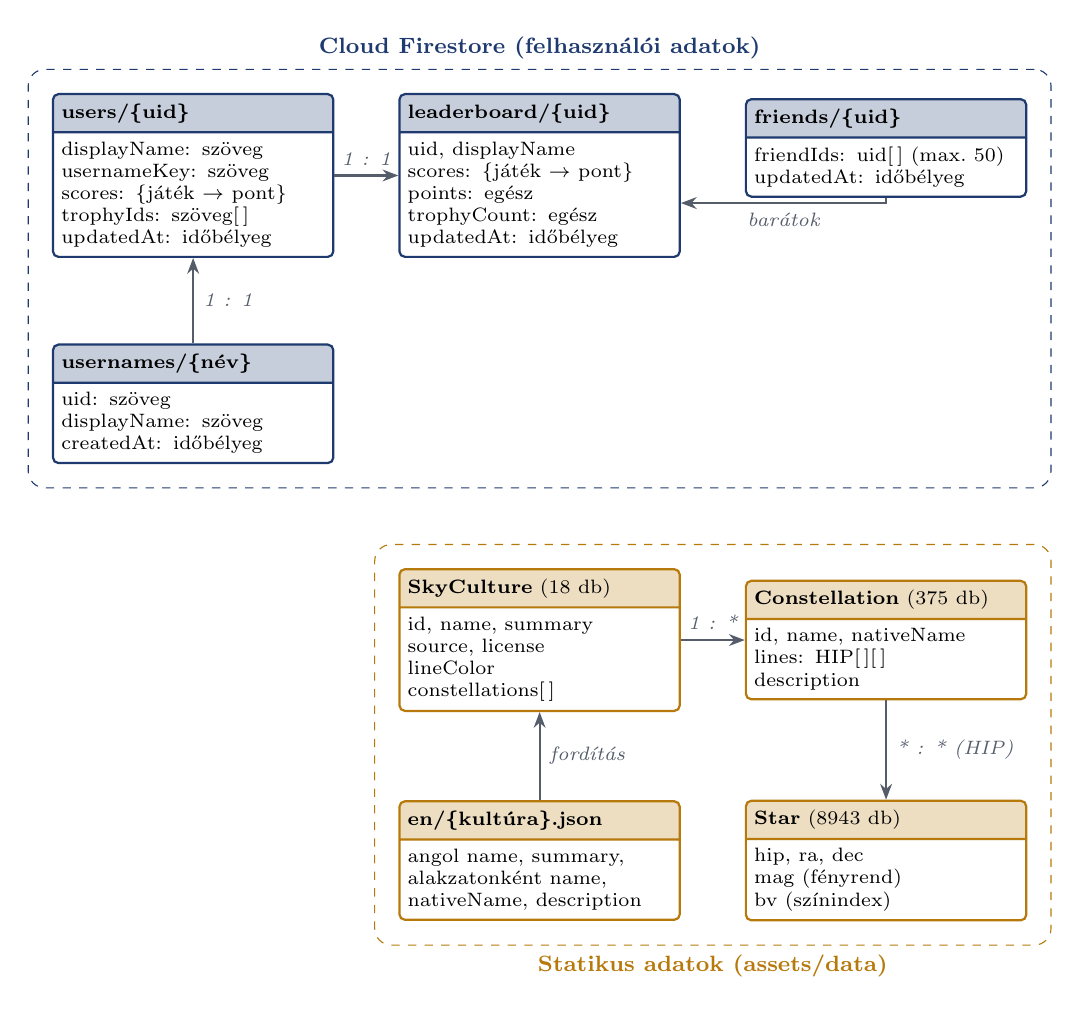
\begin{tikzpicture}[
      tabla/.style={rectangle split,rectangle split parts=2,draw=#1,thick,rounded corners=2pt,
                    font=\scriptsize,align=left,text width=3.35cm,inner sep=3pt,
                    rectangle split part fill={#1!25,white}},
      kapcs/.style={-{Stealth[length=2mm]},thick,draw=szurke},
      cimke/.style={font=\scriptsize\itshape,text=szurke}]
    % Firestore
    \node[tabla=egkek] (users) at (0,0) {\textbf{users/\{uid\}}
      \nodepart{second} displayName: szöveg\\ usernameKey: szöveg\\ scores: \{játék $\to$ pont\}\\ trophyIds: szöveg[\,]\\ updatedAt: időbélyeg};
    \node[tabla=egkek] (lb) at (4.4,0) {\textbf{leaderboard/\{uid\}}
      \nodepart{second} uid, displayName\\ scores: \{játék $\to$ pont\}\\ points: egész\\ trophyCount: egész\\ updatedAt: időbélyeg};
    \node[tabla=egkek] (fr) at (8.8,0.35) {\textbf{friends/\{uid\}}
      \nodepart{second} friendIds: uid[\,] (max.~50)\\ updatedAt: időbélyeg};
    \node[tabla=egkek] (un) at (0,-2.9) {\textbf{usernames/\{név\}}
      \nodepart{second} uid: szöveg\\ displayName: szöveg\\ createdAt: időbélyeg};

    \draw[kapcs] (users) -- node[above,cimke]{1 : 1} (lb);
    \draw[kapcs] (fr.south) |- node[pos=0.75,below,cimke]{barátok} ($(lb.east)+(0,-0.35)$);
    \draw[kapcs] (un) -- node[right,cimke]{1 : 1} (users);

    % Statikus adatok
    \node[tabla=arany] (cult) at (4.4,-5.9) {\textbf{SkyCulture} (18 db)
      \nodepart{second} id, name, summary\\ source, license\\ lineColor\\ constellations[\,]};
    \node[tabla=arany] (con) at (8.8,-5.9) {\textbf{Constellation} (375 db)
      \nodepart{second} id, name, nativeName\\ lines: HIP[\,][\,]\\ description};
    \node[tabla=arany] (star) at (8.8,-8.7) {\textbf{Star} (8943 db)
      \nodepart{second} hip, ra, dec\\ mag (fényrend)\\ bv (színindex)};
    \node[tabla=arany] (en) at (4.4,-8.7) {\textbf{en/\{kultúra\}.json}
      \nodepart{second} angol name, summary,\\ alakzatonként name,\\ nativeName, description};
    \draw[kapcs] (cult) -- node[above,cimke]{1 : *} (con);
    \draw[kapcs] (con) -- node[right,cimke]{* : * (HIP)} (star);
    \draw[kapcs] (en) -- node[right,cimke]{fordítás} (cult);

    \begin{scope}[on background layer]
      \node[fit=(users)(lb)(fr)(un),draw=egkek,dashed,rounded corners=6pt,inner sep=0.3cm,
            label={[font=\footnotesize\bfseries,text=egkek]above:Cloud Firestore (felhasználói adatok)}] {};
      \node[fit=(cult)(con)(star)(en),draw=arany,dashed,rounded corners=6pt,inner sep=0.3cm,
            label={[font=\footnotesize\bfseries,text=arany]below:Statikus adatok (assets/data)}] {};
    \end{scope}
  \end{tikzpicture}
  \caption{Adatmodell}
  \label{fig:adatmodell}
\end{figure}

\textbf{users:} a felhasználó saját, csak általa olvasható és írható profilja: megjelenített név,
a játékonkénti legjobb pontszámok és a megszerzett trófeák.

\textbf{leaderboard:} a nyilvános ranglista-bejegyzés, amelyet mindenki olvashat, de csak a
tulajdonosa írhat. Csak a megjelenítéshez szükséges adatokat tartalmazza (e-mail-címet nem); a
biztonsági szabályok ellenőrzik a mezők körét és típusát, valamint azt, hogy a pontszámok
nemnegatív egészek legyenek.

\textbf{friends:} a felhasználó barátainak azonosítói (legfeljebb 50). A barátok adatai a
nyilvános ranglista-bejegyzésekből jönnek.

\textbf{usernames:} a lefoglalt felhasználónevek, a név kisbetűs alakja szerint. A foglalás
tranzakcióban történik, ami garantálja a nevek egyediségét.

\subsection{Projektmenedzsment - GitHub}

A fejlesztés során a közös munkát GitHubon szerveztük. A feladatokat issue-kban rögzítettük, és
mindegyik új funkció külön ágon (\emph{feature branch}) készült, például
\kod{feature/egbolt}, \kod{feature/multiple-cultures}, \kod{feature/hiedel-talalojatek},
\kod{leaderboard} vagy \kod{logging}. Az elkészült munka pull requesten keresztül került a fő
ágba, miután a csapat átnézte és kipróbálta. A projekt 2026 októberének elejétől november végéig
tartott; a fontosabb mérföldköveket a \ref{fig:idovonal}.~ábra mutatja.

\begin{figure}[H]
  \centering
  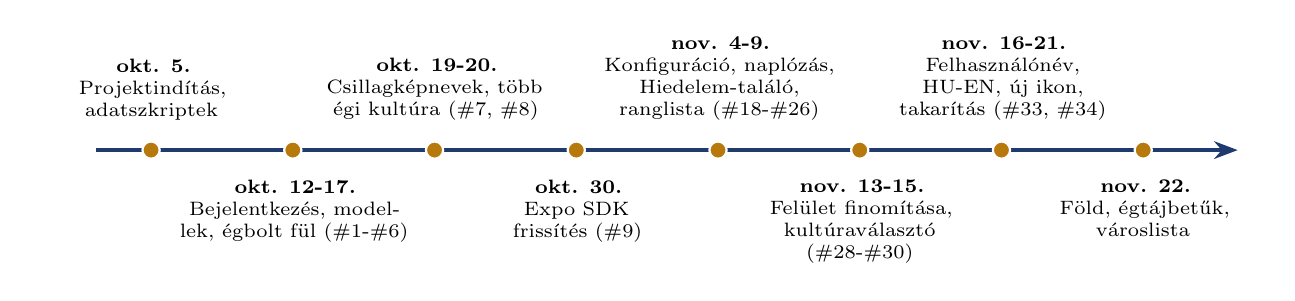
\begin{tikzpicture}[
      pont/.style={circle,fill=arany,draw=white,thick,inner sep=2.2pt},
      esem/.style={font=\scriptsize,align=center,text width=2.9cm}]
    \draw[very thick,egkek,-{Stealth[length=3mm]}] (0.7,0) -- (15.2,0);
    \node[pont] at (1.40,0) {};
    \node[esem,anchor=south] at (1.40,0.25) {\textbf{okt. 5.}\\ Projektindítás, adatszkriptek};
    \node[pont] at (3.20,0) {};
    \node[esem,anchor=north] at (3.20,-0.25) {\textbf{okt. 12-17.}\\ Bejelentkezés, modellek, égbolt fül (\#1-\#6)};
    \node[pont] at (5.00,0) {};
    \node[esem,anchor=south] at (5.00,0.25) {\textbf{okt. 19-20.}\\ Csillagképnevek, több égi kultúra (\#7, \#8)};
    \node[pont] at (6.80,0) {};
    \node[esem,anchor=north] at (6.80,-0.25) {\textbf{okt. 30.}\\ Expo SDK frissítés (\#9)};
    \node[pont] at (8.60,0) {};
    \node[esem,anchor=south] at (8.60,0.25) {\textbf{nov. 4-9.}\\ Konfiguráció, naplózás, Hiedelem-találó, ranglista (\#18-\#26)};
    \node[pont] at (10.40,0) {};
    \node[esem,anchor=north] at (10.40,-0.25) {\textbf{nov. 13-15.}\\ Felület finomítása, kultúraválasztó (\#28-\#30)};
    \node[pont] at (12.20,0) {};
    \node[esem,anchor=south] at (12.20,0.25) {\textbf{nov. 16-21.}\\ Felhasználónév, HU-EN, új ikon, takarítás (\#33, \#34)};
    \node[pont] at (14.00,0) {};
    \node[esem,anchor=north] at (14.00,-0.25) {\textbf{nov. 22.}\\ Föld, égtájbetűk, városlista};
  \end{tikzpicture}
  \caption{A fejlesztés fő mérföldkövei (a számok a pull requesteket jelölik)}
  \label{fig:idovonal}
\end{figure}

% =====================================================================
\section{Alkalmazás működése}

\subsection{UI - konkrét megvalósítás}

A felhasználói felület kialakításánál a letisztultságra, az egységes megjelenésre és a könnyű
kezelhetőségre törekedtünk. A felület sötét, éjkék alapszínű (hogy éjszakai használatnál ne
vakítson), a kiemelések arany színűek, a panelek áttetsző, „üveghatású” felületek. Az elrendezés
a képernyő méretéhez igazodik: asztali nézetben bal oldali menüsáv, tableten lebegő menü,
telefonon az alsó ikonsáv és ujjal lapozható oldalak segítik a navigációt. Az alábbi
képernyőképek a webes változatból, helyi (bemutató) módban készültek.

\begin{figure}[H]
  \centering
  \begin{subfigure}[t]{0.49\linewidth}
    \centering
    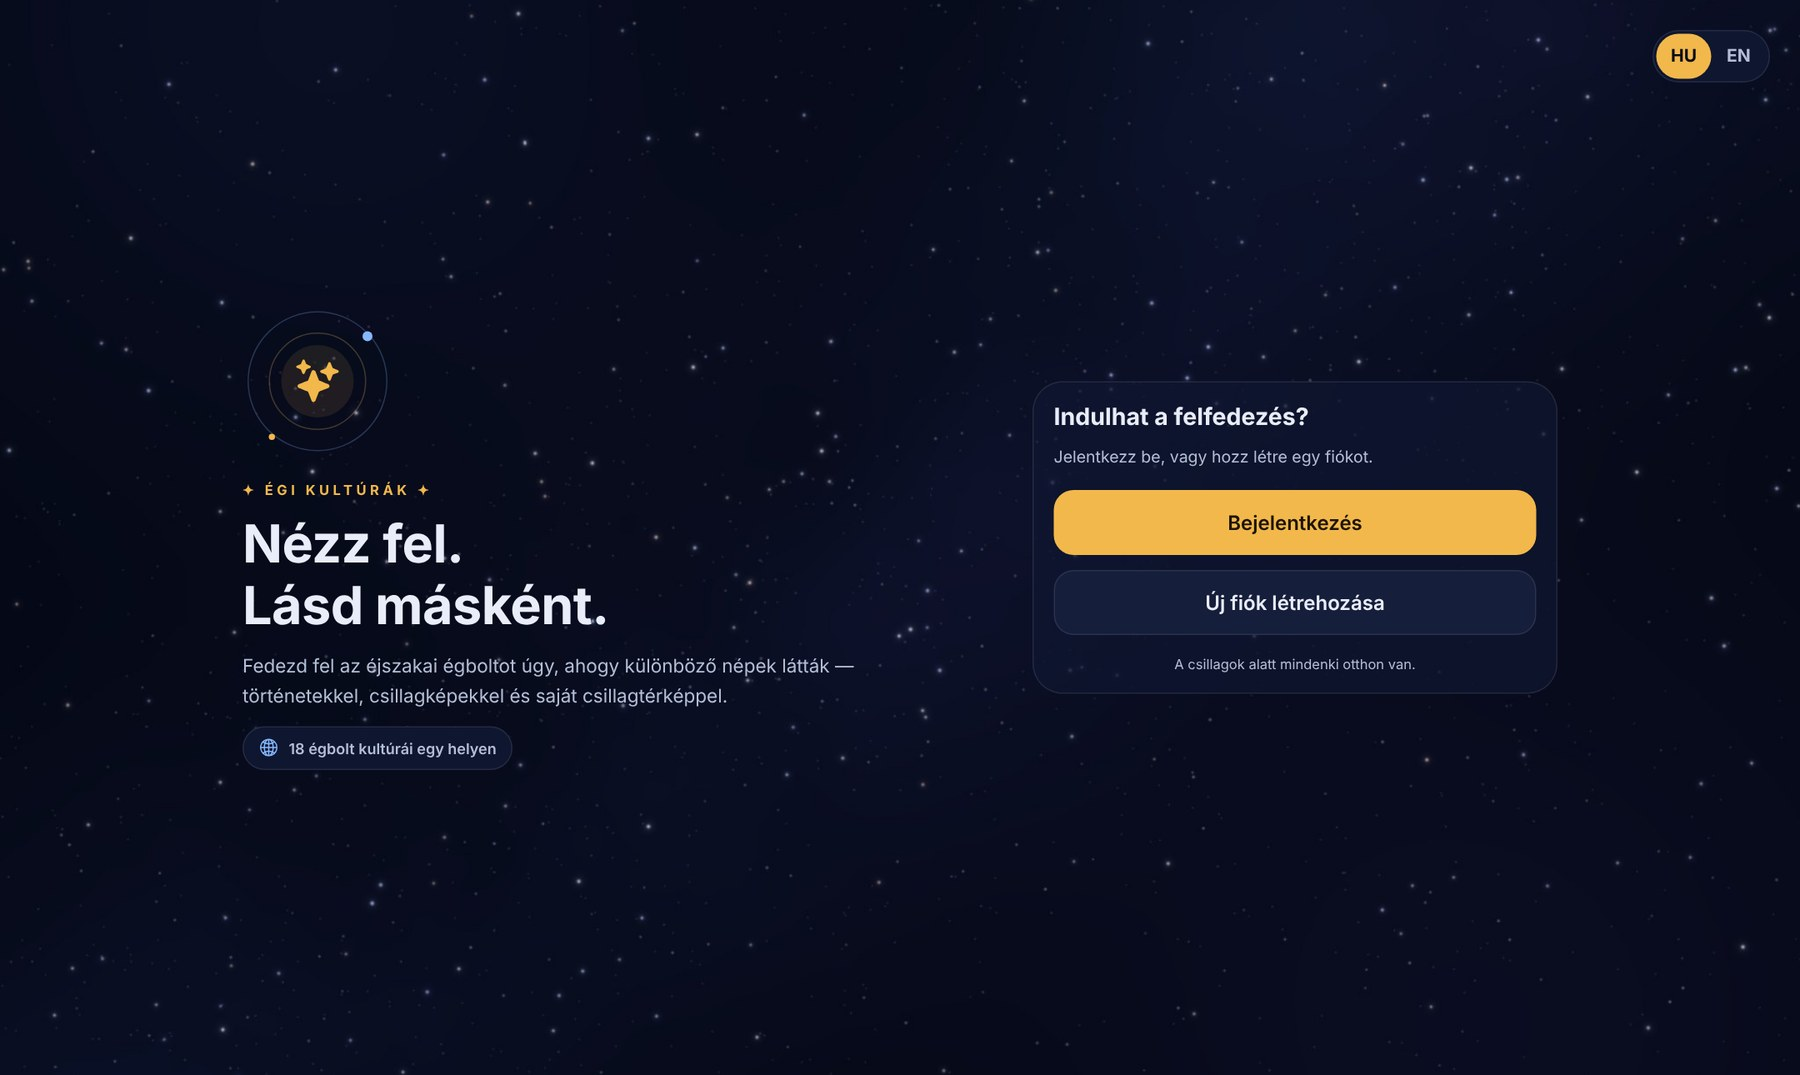
\includegraphics[width=\linewidth]{kepek/kezdokepernyo.jpg}
    \caption{Kezdőképernyő}
  \end{subfigure}\hfill
  \begin{subfigure}[t]{0.49\linewidth}
    \centering
    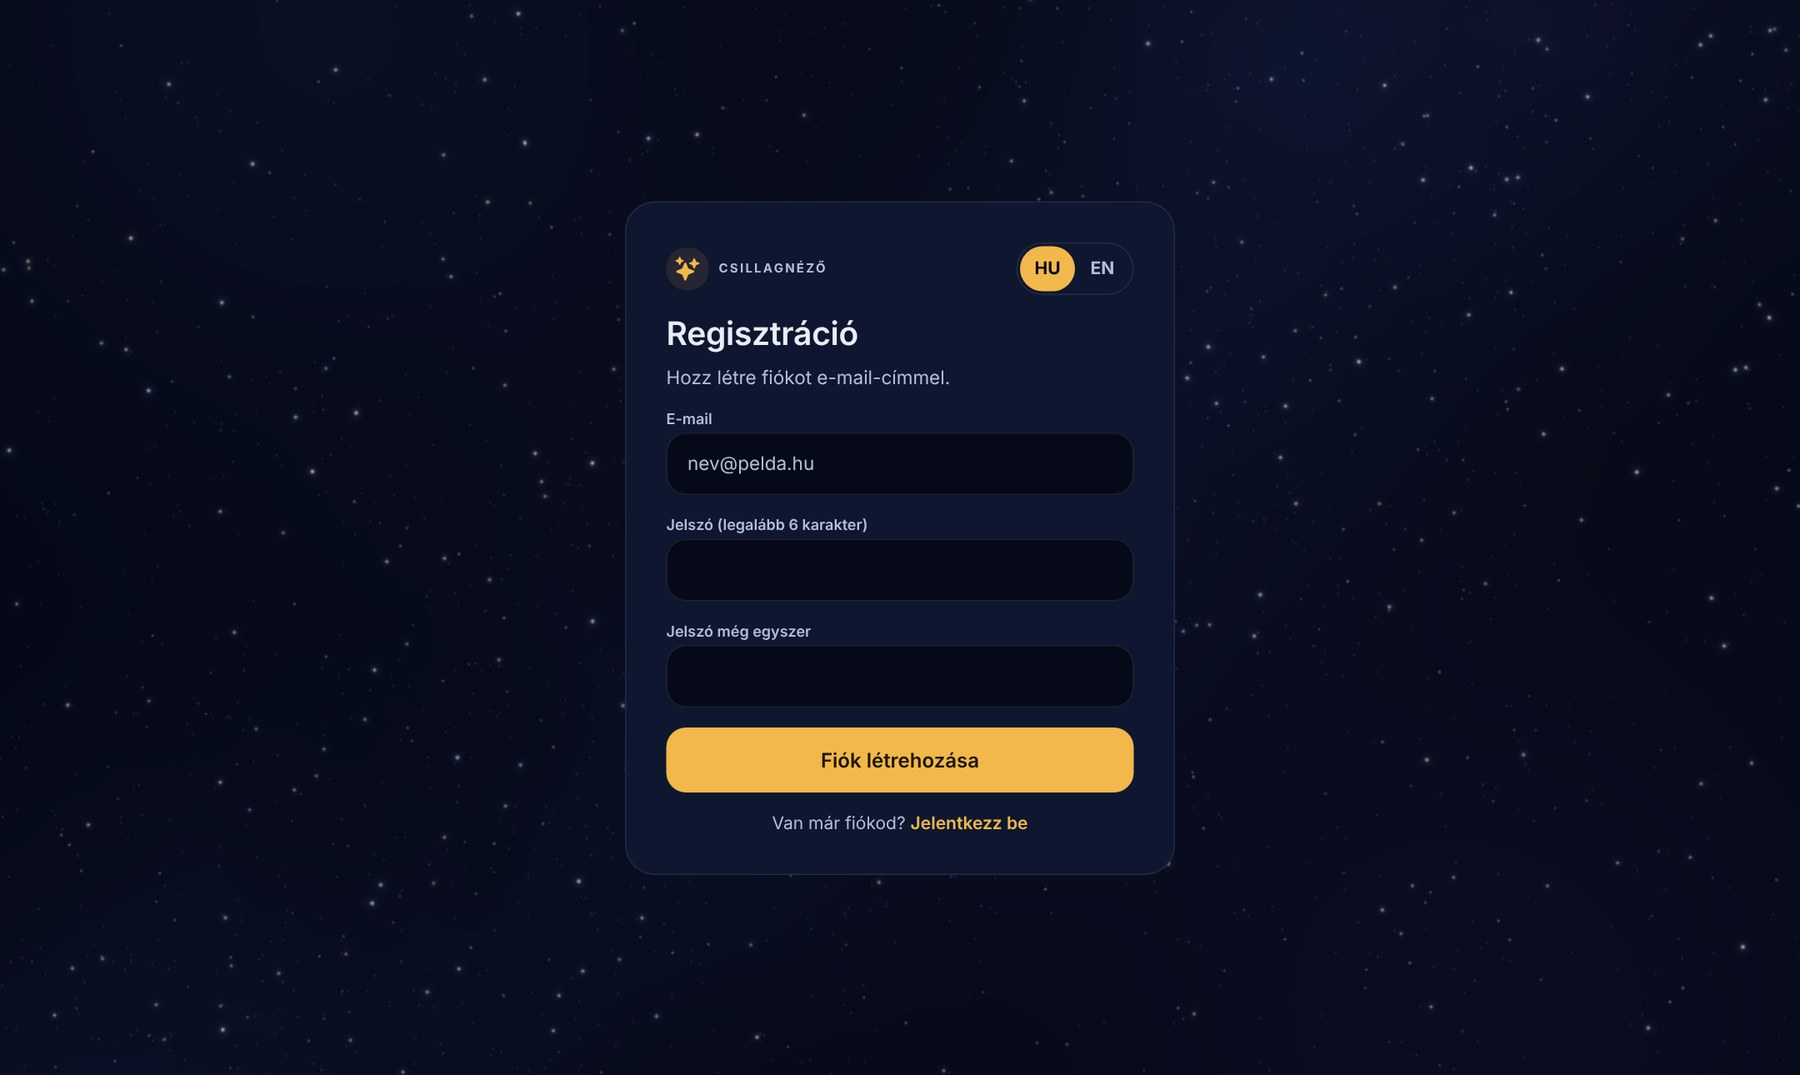
\includegraphics[width=\linewidth]{kepek/regisztracio.jpg}
    \caption{Regisztráció}
  \end{subfigure}
  \caption{Kezdőképernyő és regisztráció}
  \label{fig:kezdo}
\end{figure}

\textbf{Kezdőképernyő és regisztráció:} bejelentkezés nélkül ez a képernyő fogadja a
felhasználót (\ref{fig:kezdo}.~ábra). Innen jut el a bejelentkezéshez vagy az új fiók létrehozásához, a jobb felső
sarokban pedig nyelvet válthat. Az űrlapok helyben ellenőrzik a megadott adatokat (e-mail-cím
formátuma, jelszó hossza, a két jelszó egyezése).

\begin{figure}[H]
  \centering
  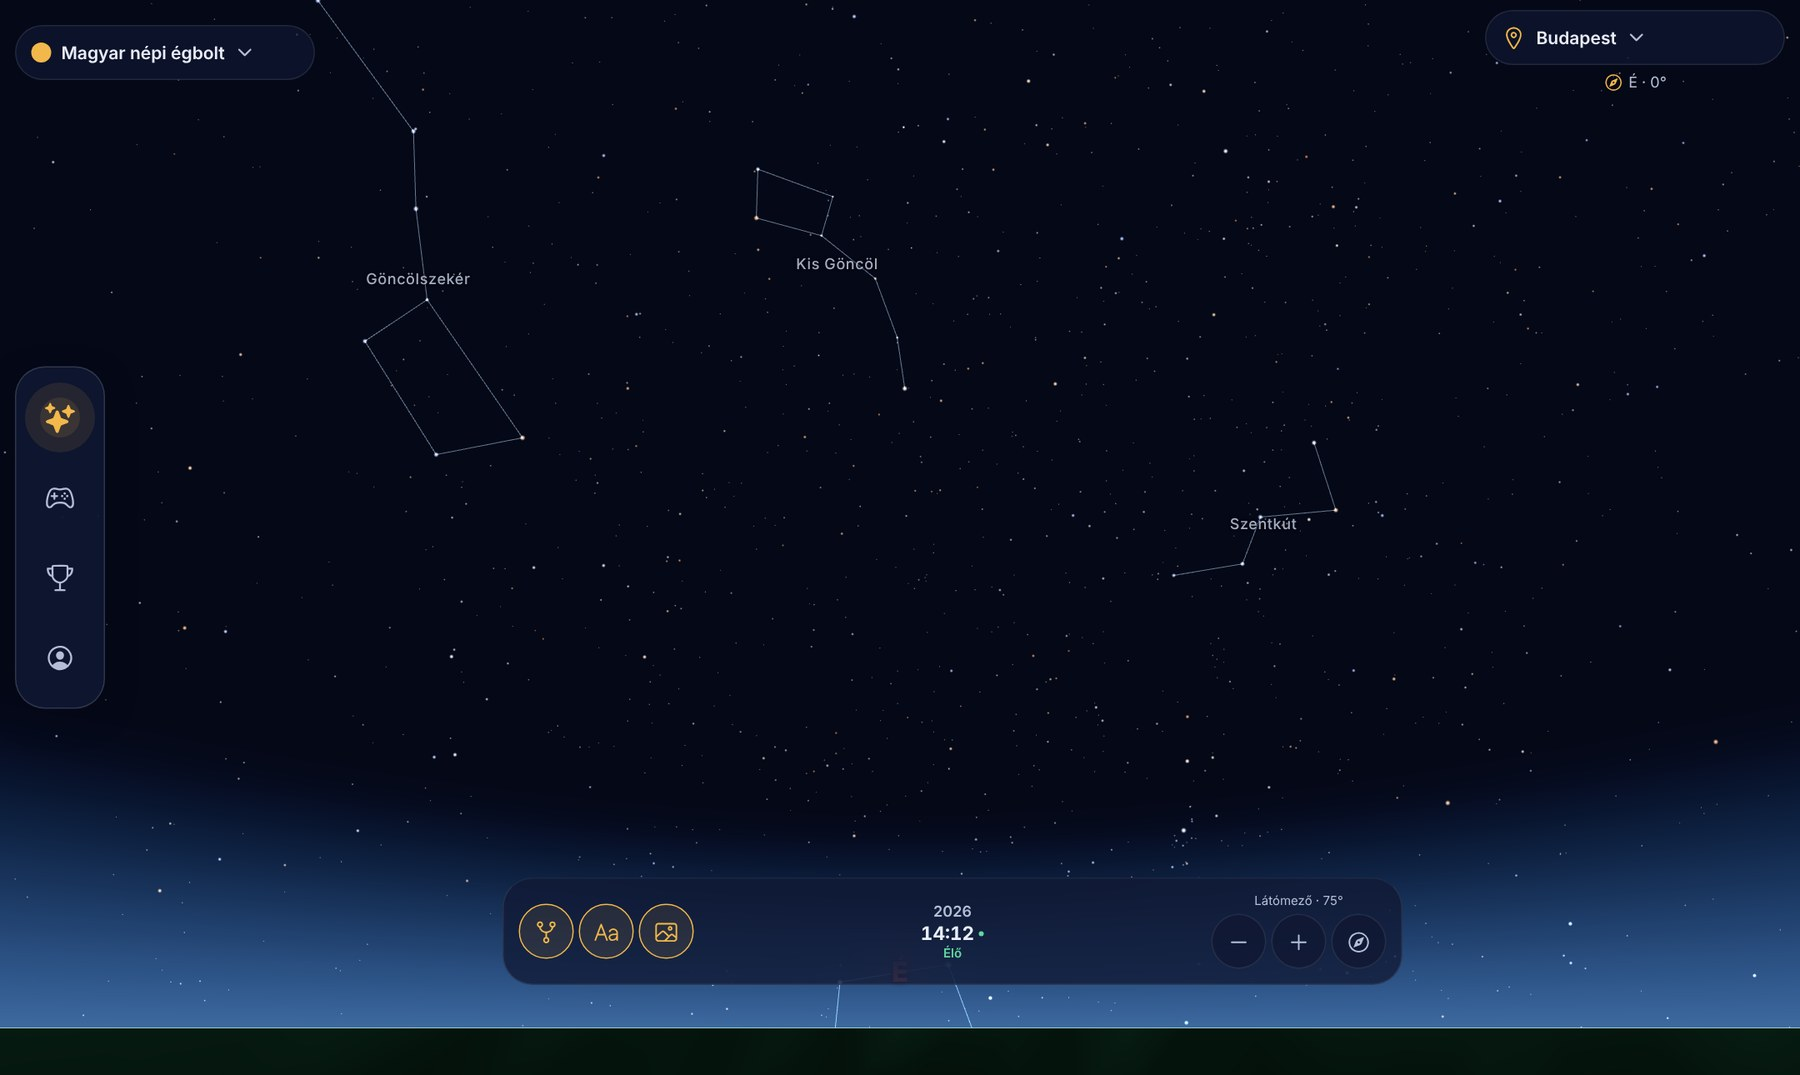
\includegraphics[width=0.82\linewidth]{kepek/elo-egbolt.jpg}
  \caption{Az élő égbolt (asztali nézet, magyar népi égbolt, Budapest)}
  \label{fig:elo}
\end{figure}

\textbf{Élő égbolt:} az alkalmazás központi képernyője (\ref{fig:elo}.~ábra). Bal felül az égi
kultúra, jobb felül a megfigyelési hely választója és az aktuális nézési irány látható. Az alsó
dokkon a vonalak, a nevek és a föld kapcsolói, középen az aktuális időpont (az „Élő” jelzés
mutatja, hogy a valós időt követi), jobbra a látómező, a nagyítás és az alapnézet gombja
található. A horizont alatt a föld, fölötte halvány derengés és az égtájak betűi segítik a
tájékozódást.

\begin{figure}[H]
  \centering
  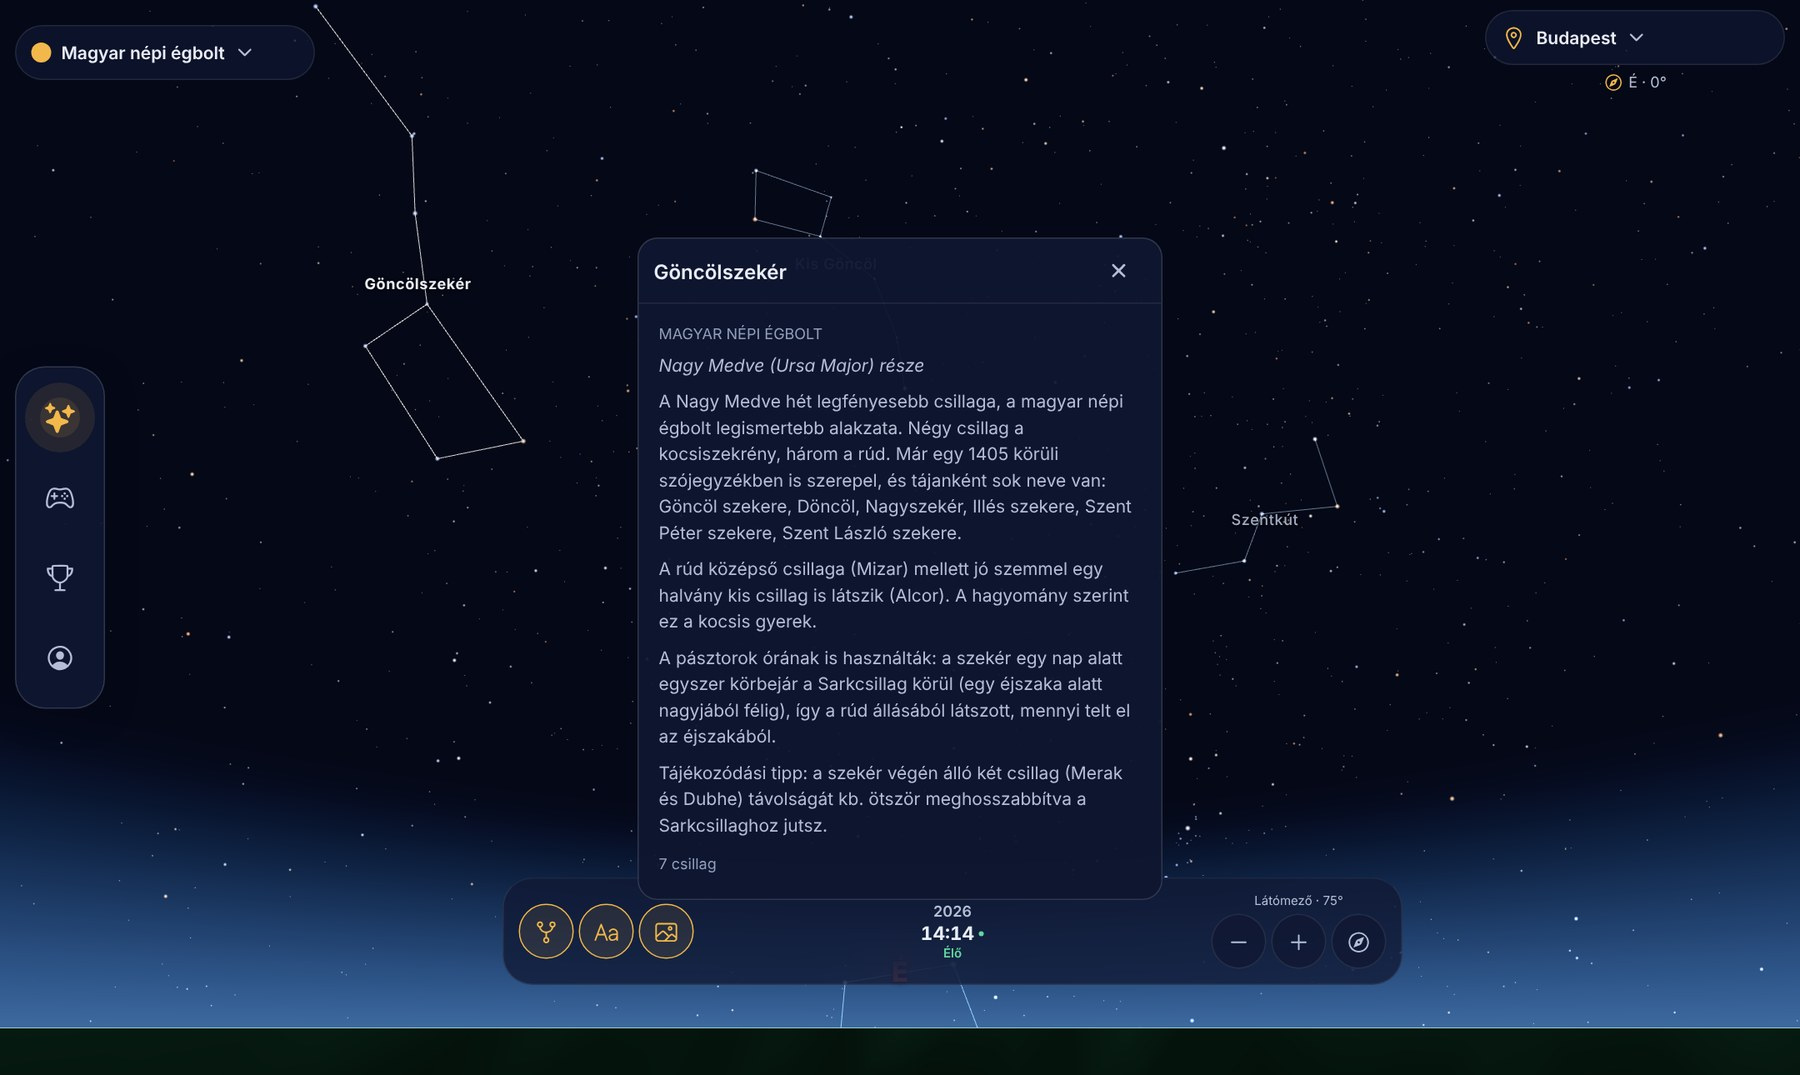
\includegraphics[width=0.82\linewidth]{kepek/csillagkep-leiras.jpg}
  \caption{Egy kiválasztott csillagkép leírása}
  \label{fig:leiras}
\end{figure}

\textbf{Csillagkép-leírás:} egy csillagképre koppintva az alakzat kiemelődik, és megnyílik a
hozzá tartozó leírás (\ref{fig:leiras}.~ábra): a kultúra neve, az alakzat eredeti vagy
csillagászati megfelelője, a legenda és a csillagok száma. Telefonon a lap alulról csúszik be,
és lefelé húzva bezárható.

\begin{figure}[H]
  \centering
  \begin{subfigure}[t]{0.49\linewidth}
    \centering
    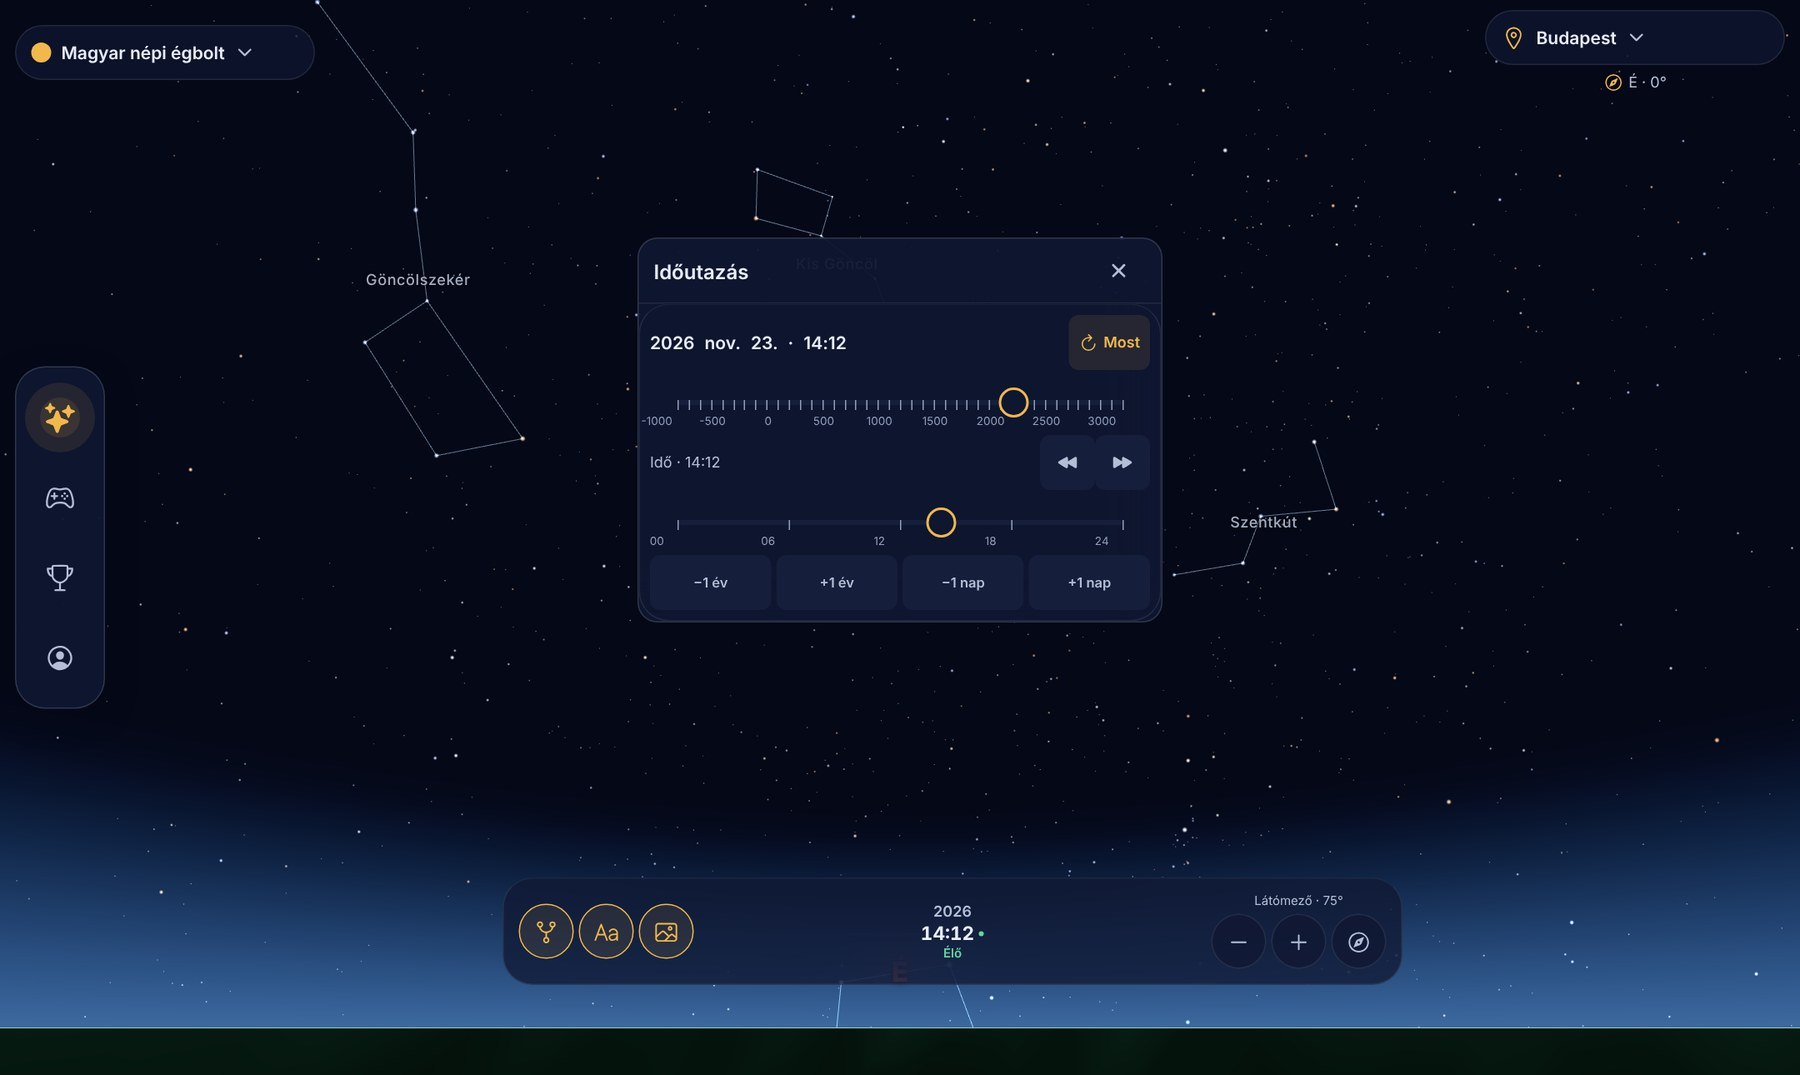
\includegraphics[width=\linewidth]{kepek/idoutazas.jpg}
    \caption{Időutazás panel}
  \end{subfigure}\hfill
  \begin{subfigure}[t]{0.49\linewidth}
    \centering
    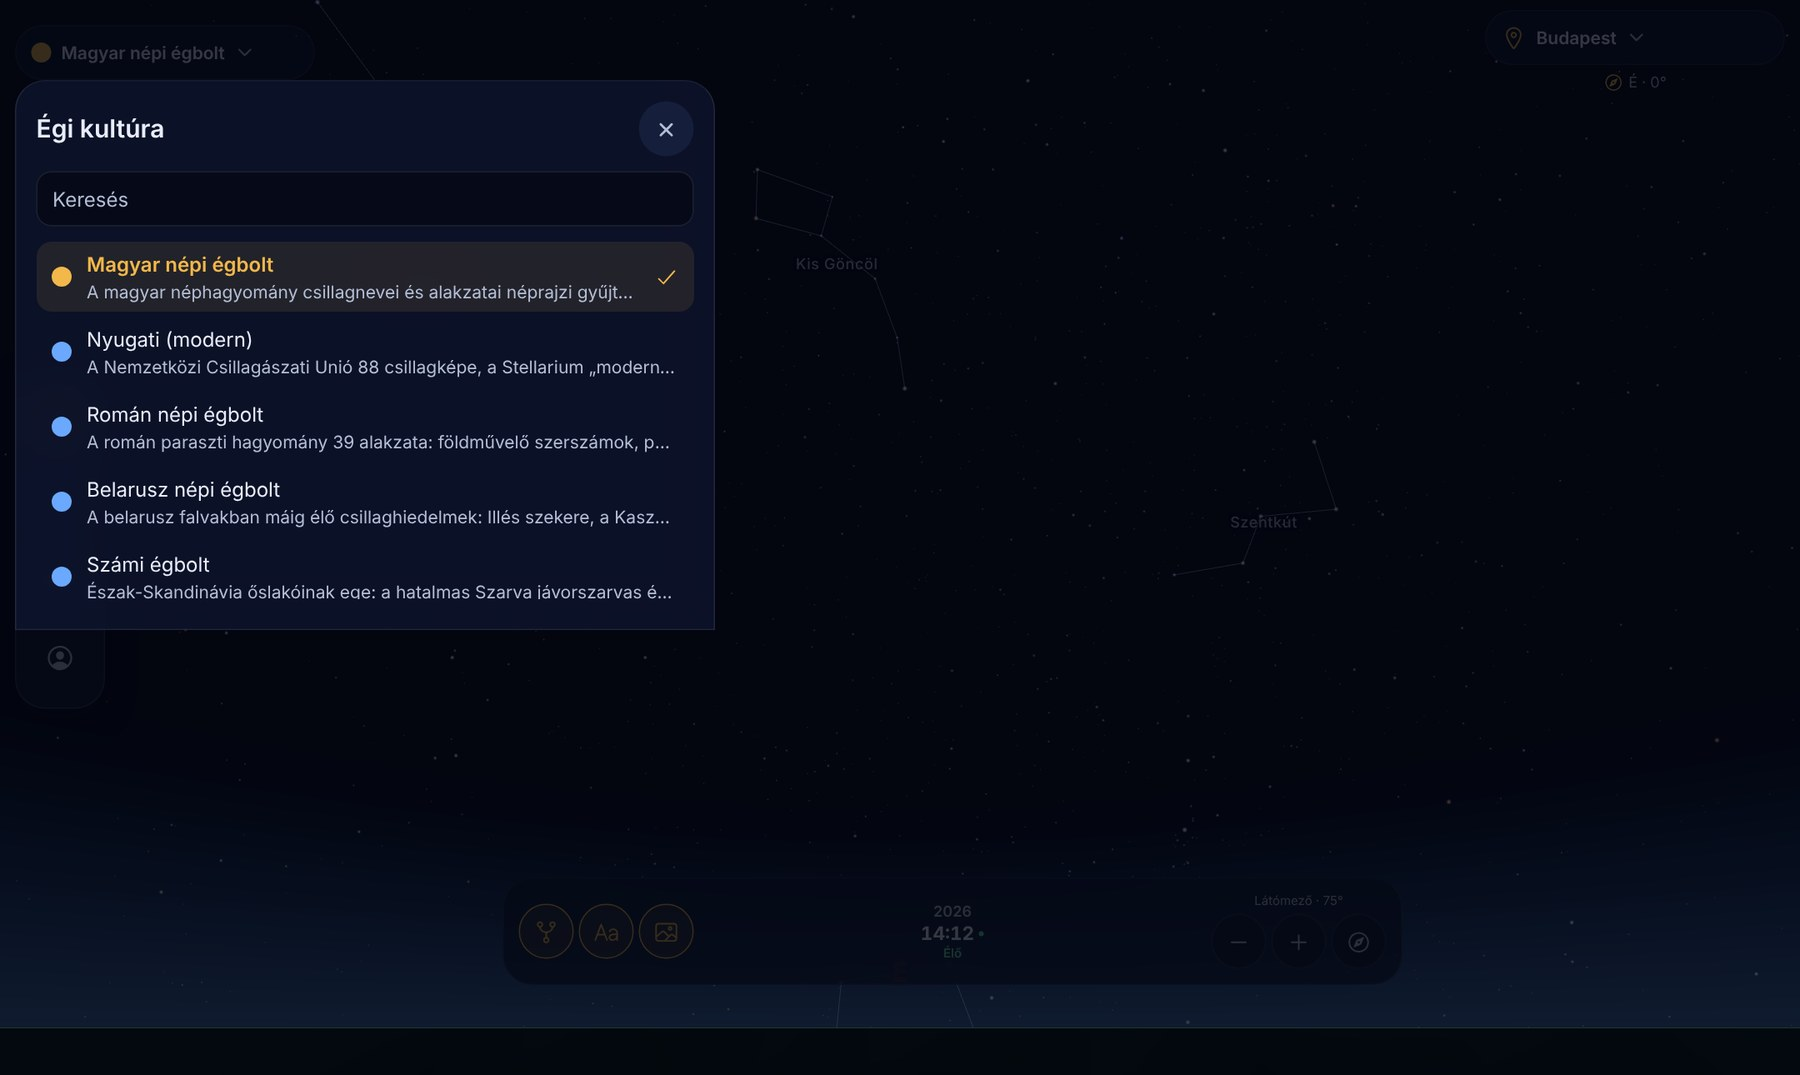
\includegraphics[width=\linewidth]{kepek/kulturavalaszto.jpg}
    \caption{Égi kultúra választása}
  \end{subfigure}
  \caption{Az időpont és az égi kultúra kiválasztása}
  \label{fig:ido-kultura}
\end{figure}

\textbf{Időutazás és kultúraválasztás:} az időutazás panelen (\ref{fig:ido-kultura}.~ábra) egy
évcsúszkával i.\,e.\ 1001 és i.\,sz.\ 3000 között, egy másik csúszkával a napon belül lehet
időt választani, a gombok egy nappal vagy egy évvel léptetnek, a „Most” gomb pedig visszaállítja
a valós időt. A kultúraválasztó kereshető listája minden kultúrához rövid bemutatást is ad.

\begin{figure}[H]
  \centering
  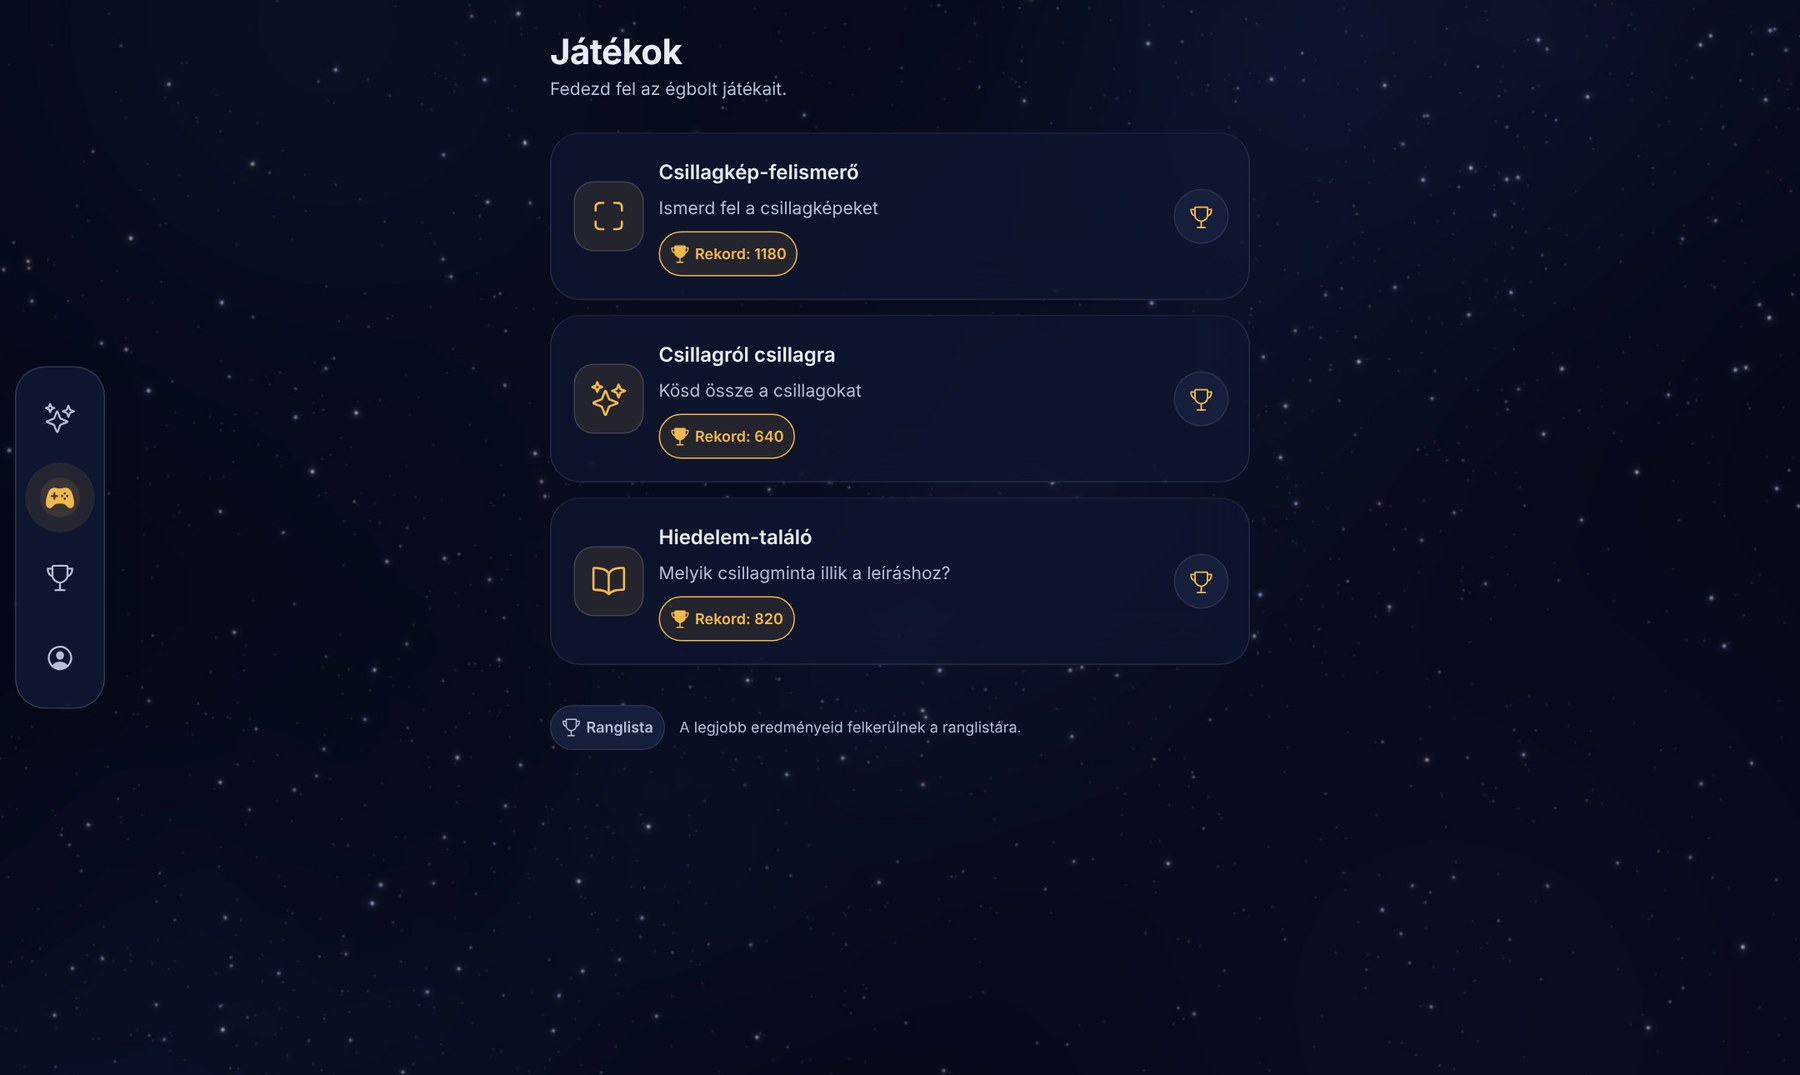
\includegraphics[width=0.82\linewidth]{kepek/jatekok.jpg}
  \caption{A Játékok képernyő}
  \label{fig:jatekok}
\end{figure}

\textbf{Játékok:} a Játékok fülön a három játék kártyái láthatók, mindegyiken a felhasználó
eddigi rekordjával (\ref{fig:jatekok}.~ábra). A játékok teljes képernyős, görgetés nélküli
keretben futnak, a fejlécben a kör sorszámával és az aktuális pontszámmal.

\begin{figure}[H]
  \centering
  \begin{subfigure}[t]{0.49\linewidth}
    \centering
    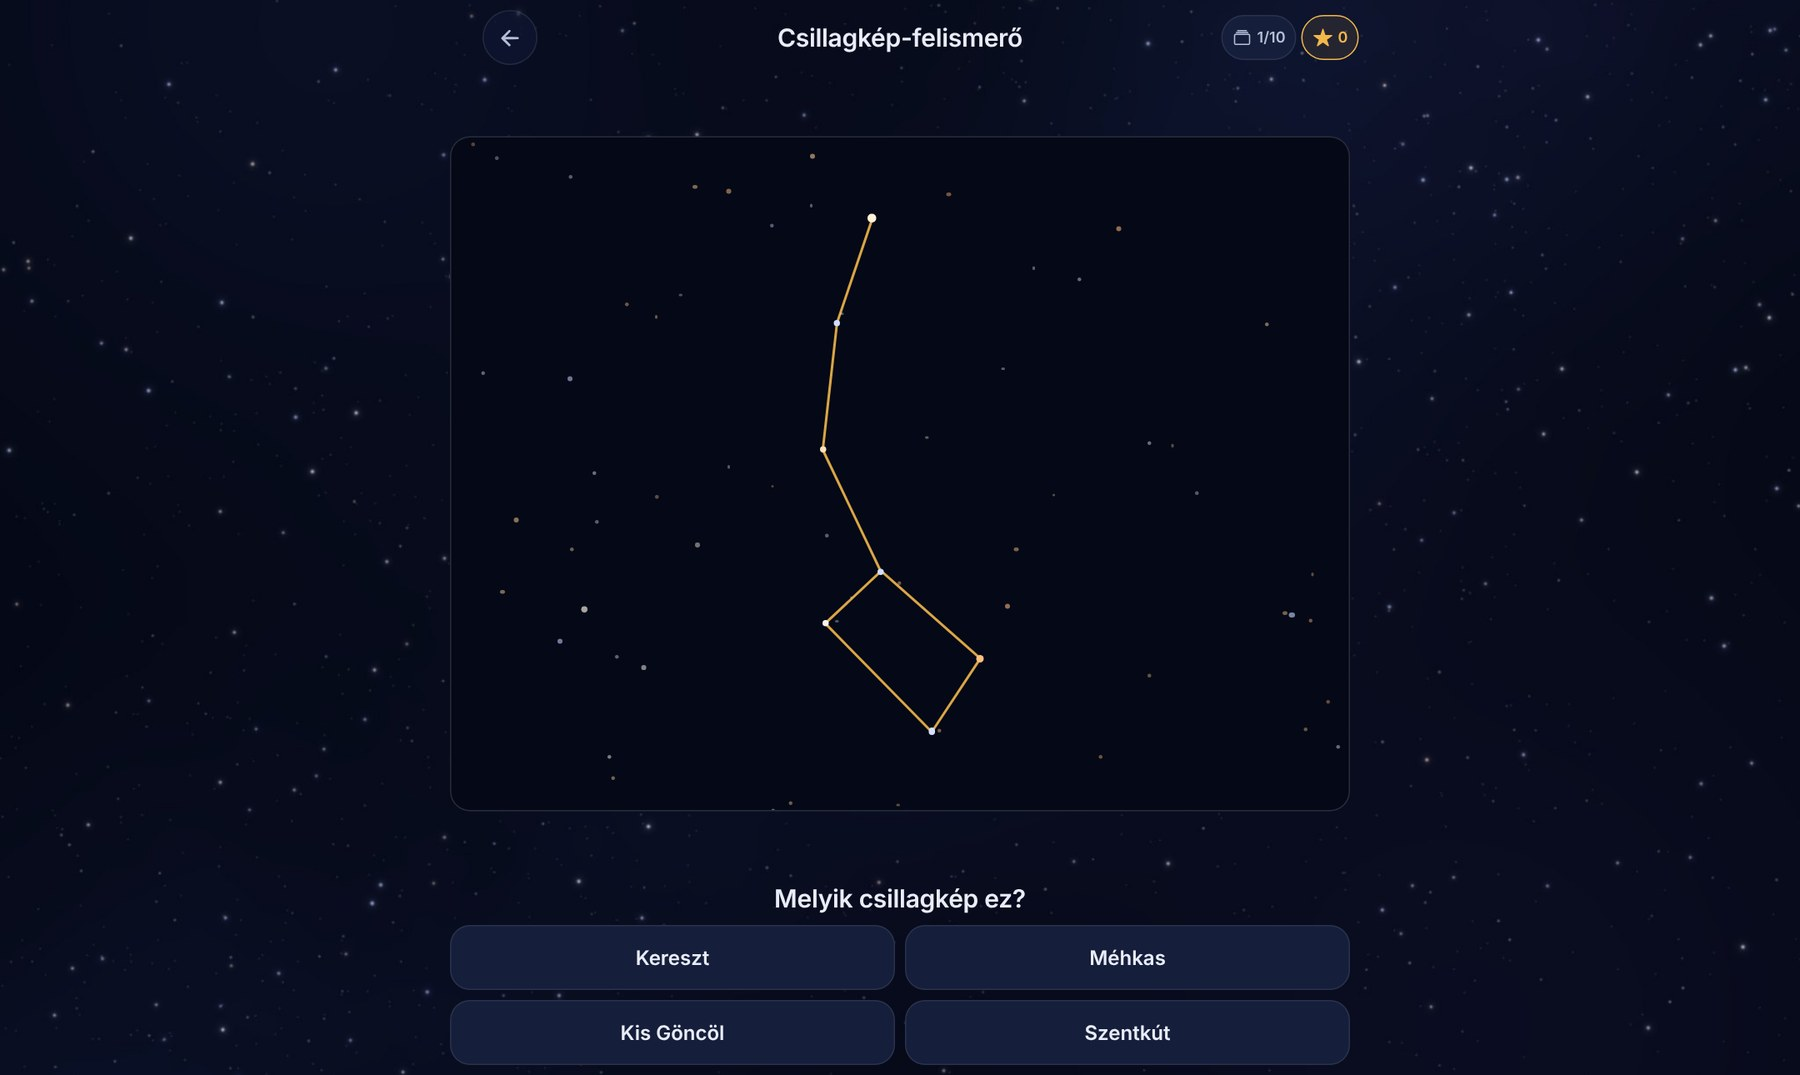
\includegraphics[width=\linewidth]{kepek/jatek-felismero.jpg}
    \caption{Csillagkép-felismerő}
  \end{subfigure}\hfill
  \begin{subfigure}[t]{0.49\linewidth}
    \centering
    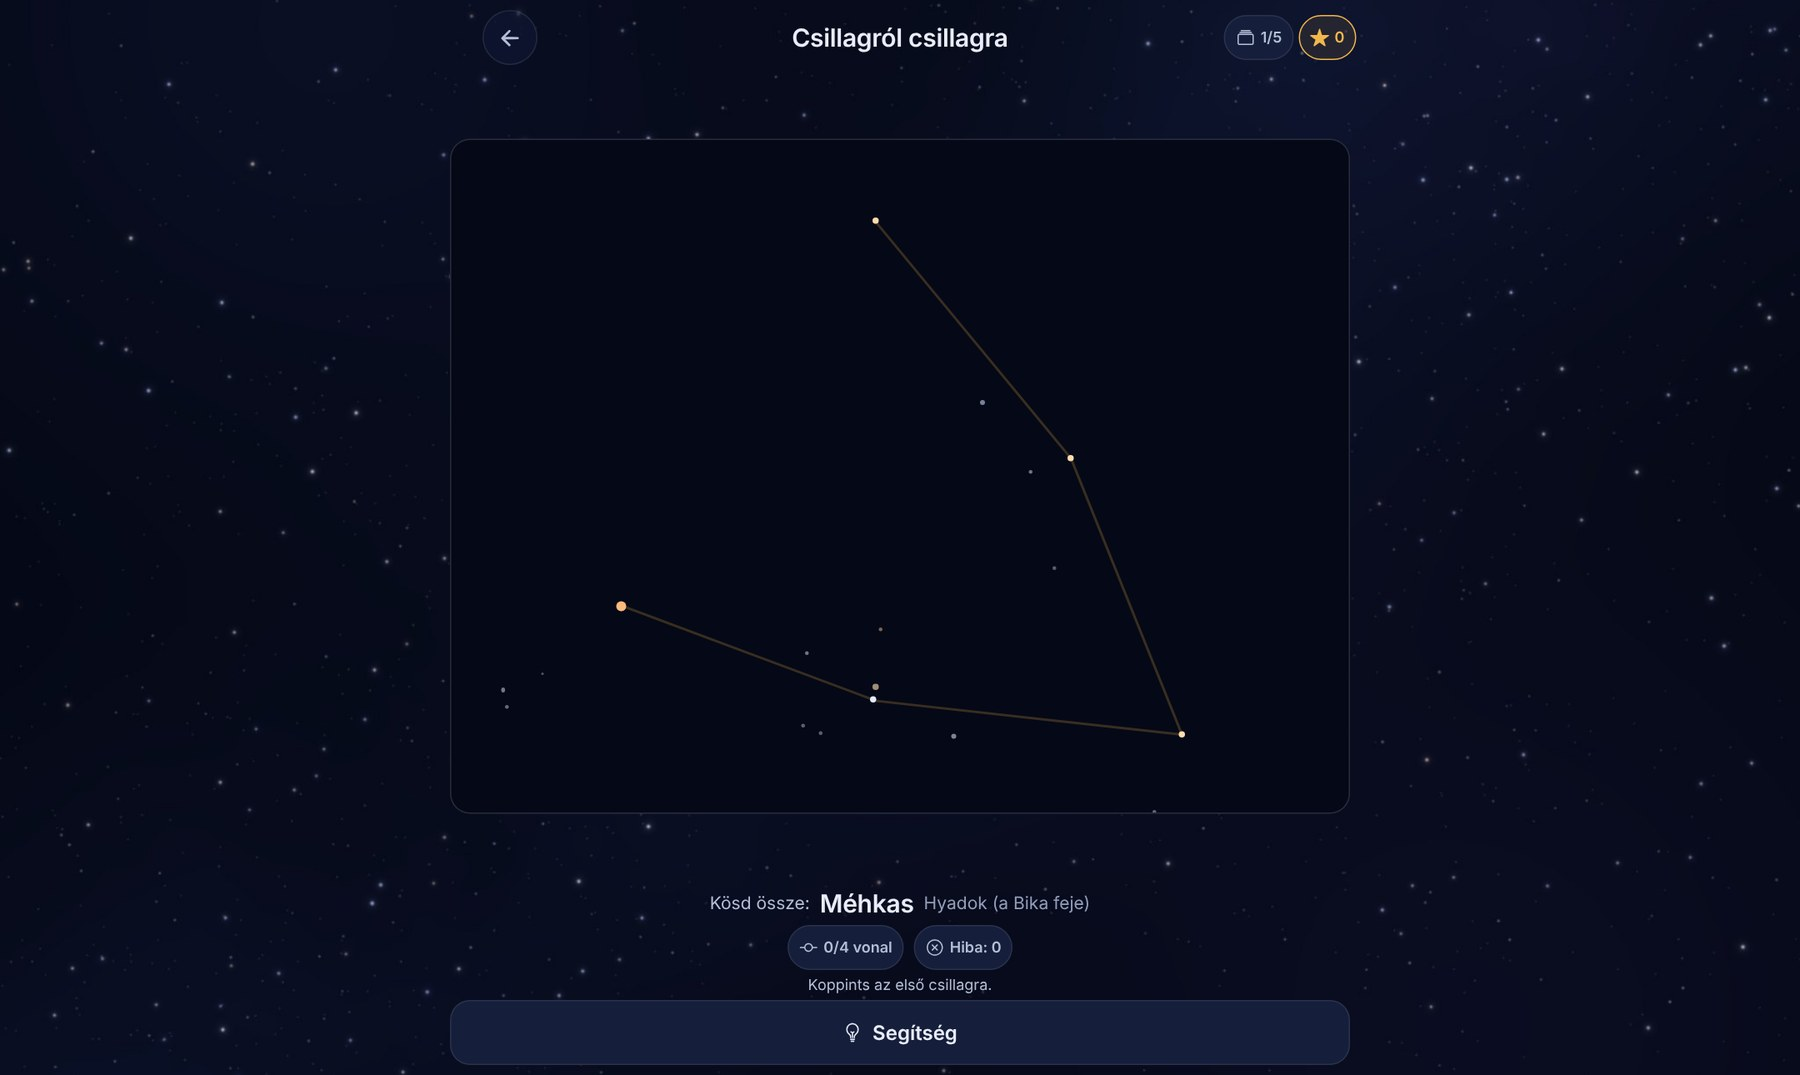
\includegraphics[width=\linewidth]{kepek/jatek-osszekoto.jpg}
    \caption{Csillagról csillagra}
  \end{subfigure}
  \caption{Két játék kérdésképernyője}
  \label{fig:jatek12}
\end{figure}

\textbf{Csillagkép-felismerő:} a játékos egy csillagképet lát, és négy név közül kell kiválasztania
a helyeset. Könnyű fokozatban a vonalak is látszanak, nehézben csak a csillagok.

\textbf{Csillagról csillagra:} a játékos megkapja egy csillagkép nevét, és a csillagokra koppintva
neki kell behúznia a vonalait. A „Segítség” gomb megmutatja a következő vonalat, de pontlevonással
jár.

\begin{figure}[H]
  \centering
  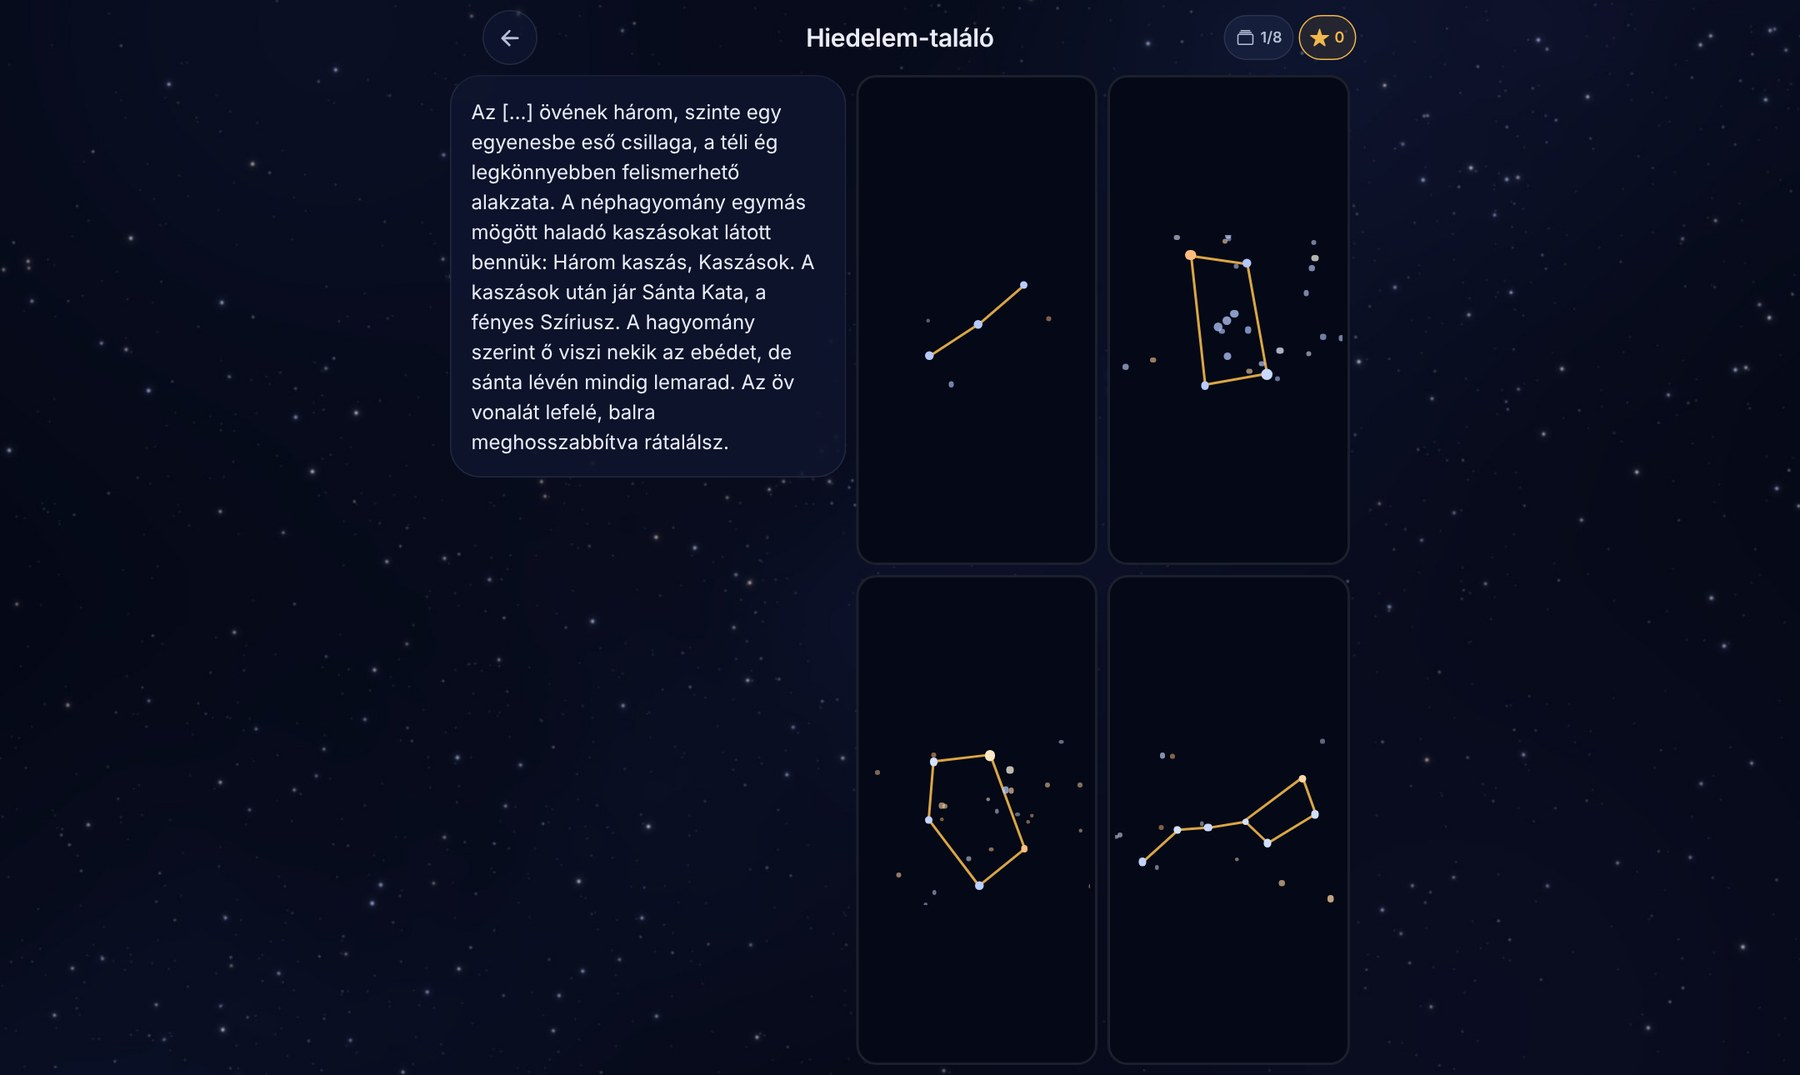
\includegraphics[width=0.82\linewidth]{kepek/jatek-hiedelem.jpg}
  \caption{A Hiedelem-találó játék}
  \label{fig:hiedelem}
\end{figure}

\textbf{Hiedelem-találó:} a játékos egy csillagképhez fűződő hiedelem vagy legenda 3-5 mondatos
leírását olvassa, és négy csillagminta közül kell kiválasztania a hozzá tartozót
(\ref{fig:hiedelem}.~ábra). A leírásban a csillagkép neve helyén „[\dots]” áll, és az
alkalmazás kiszűri azokat a mondatokat, amelyek elárulnák a választ.

\begin{figure}[H]
  \centering
  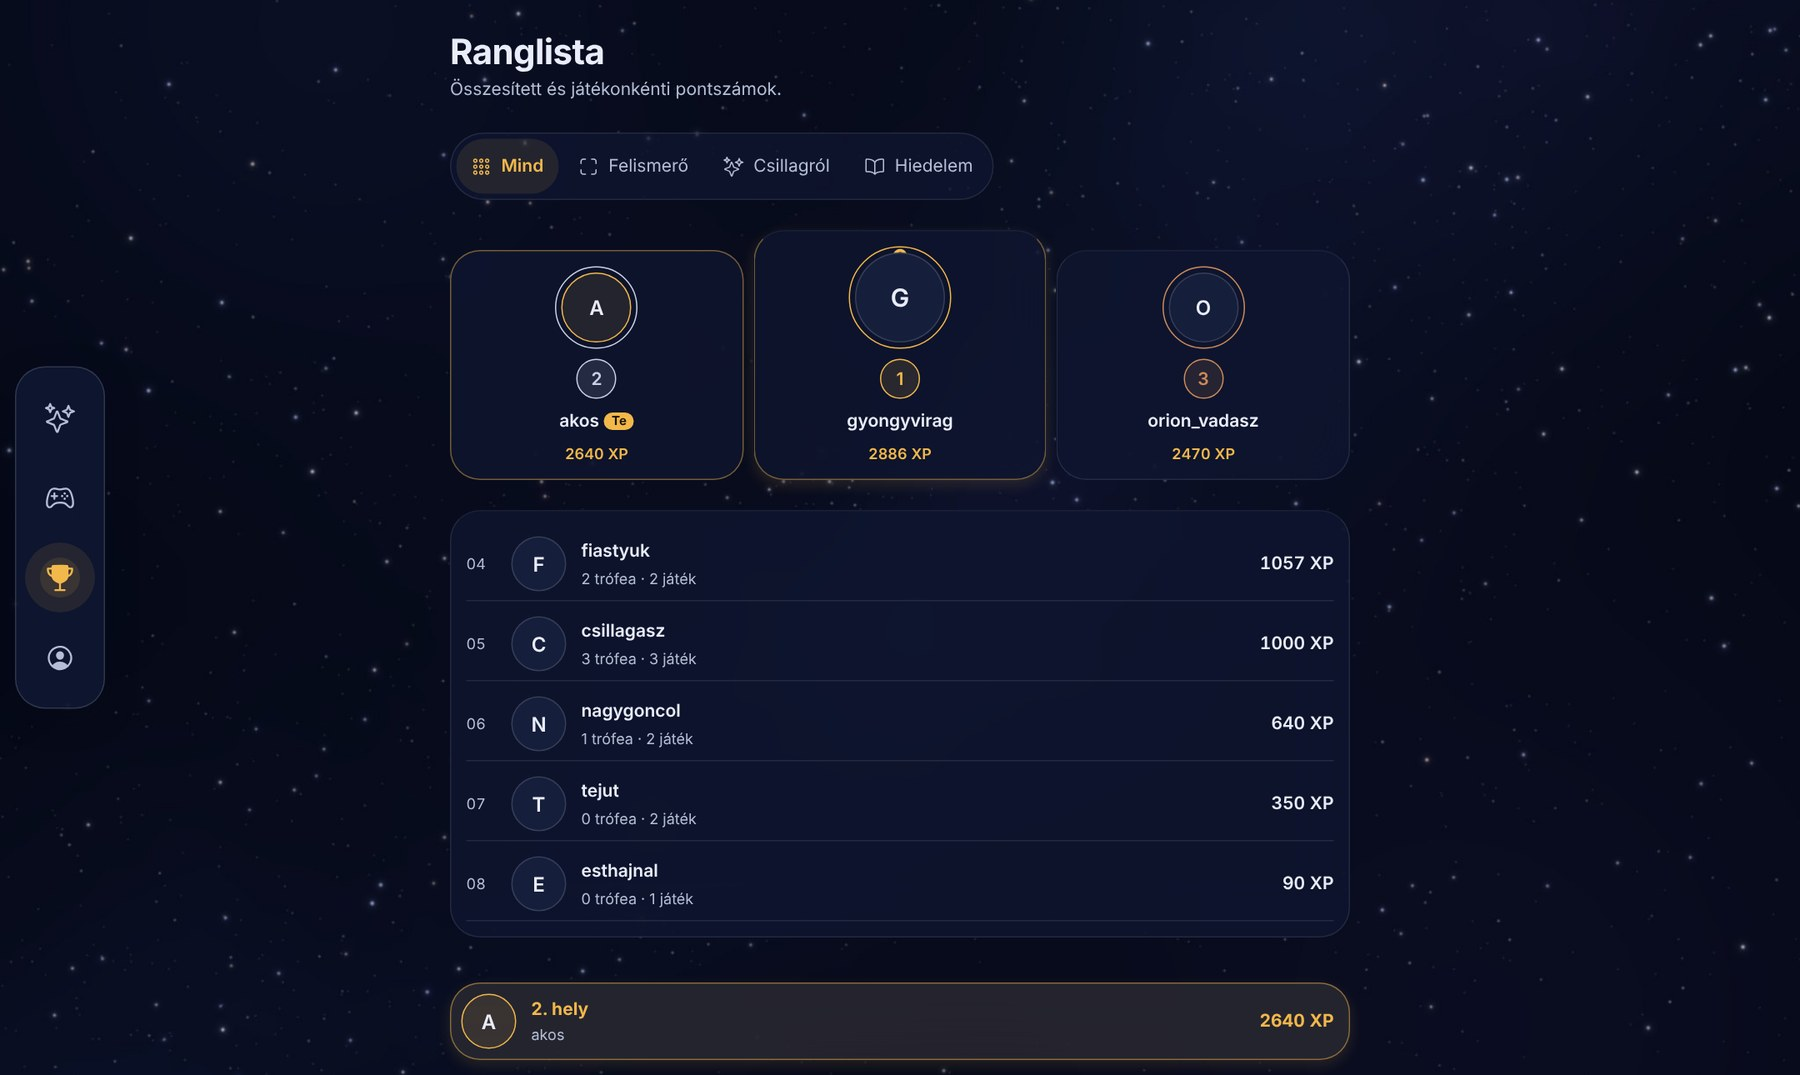
\includegraphics[width=0.82\linewidth]{kepek/ranglista.jpg}
  \caption{A ranglista}
  \label{fig:ranglista}
\end{figure}

\textbf{Ranglista:} a dobogón az első három, alatta a többi játékos látható, a pontszámmal, a
trófeák és a játszott játékok számával (\ref{fig:ranglista}.~ábra). A szűrőkkel az összesített
vagy egy-egy játék szerinti ranglista választható. A saját helyezés a lista alján mindig látszik,
kiemelve. (A képen bemutató adatok szerepelnek.)

\begin{figure}[H]
  \centering
  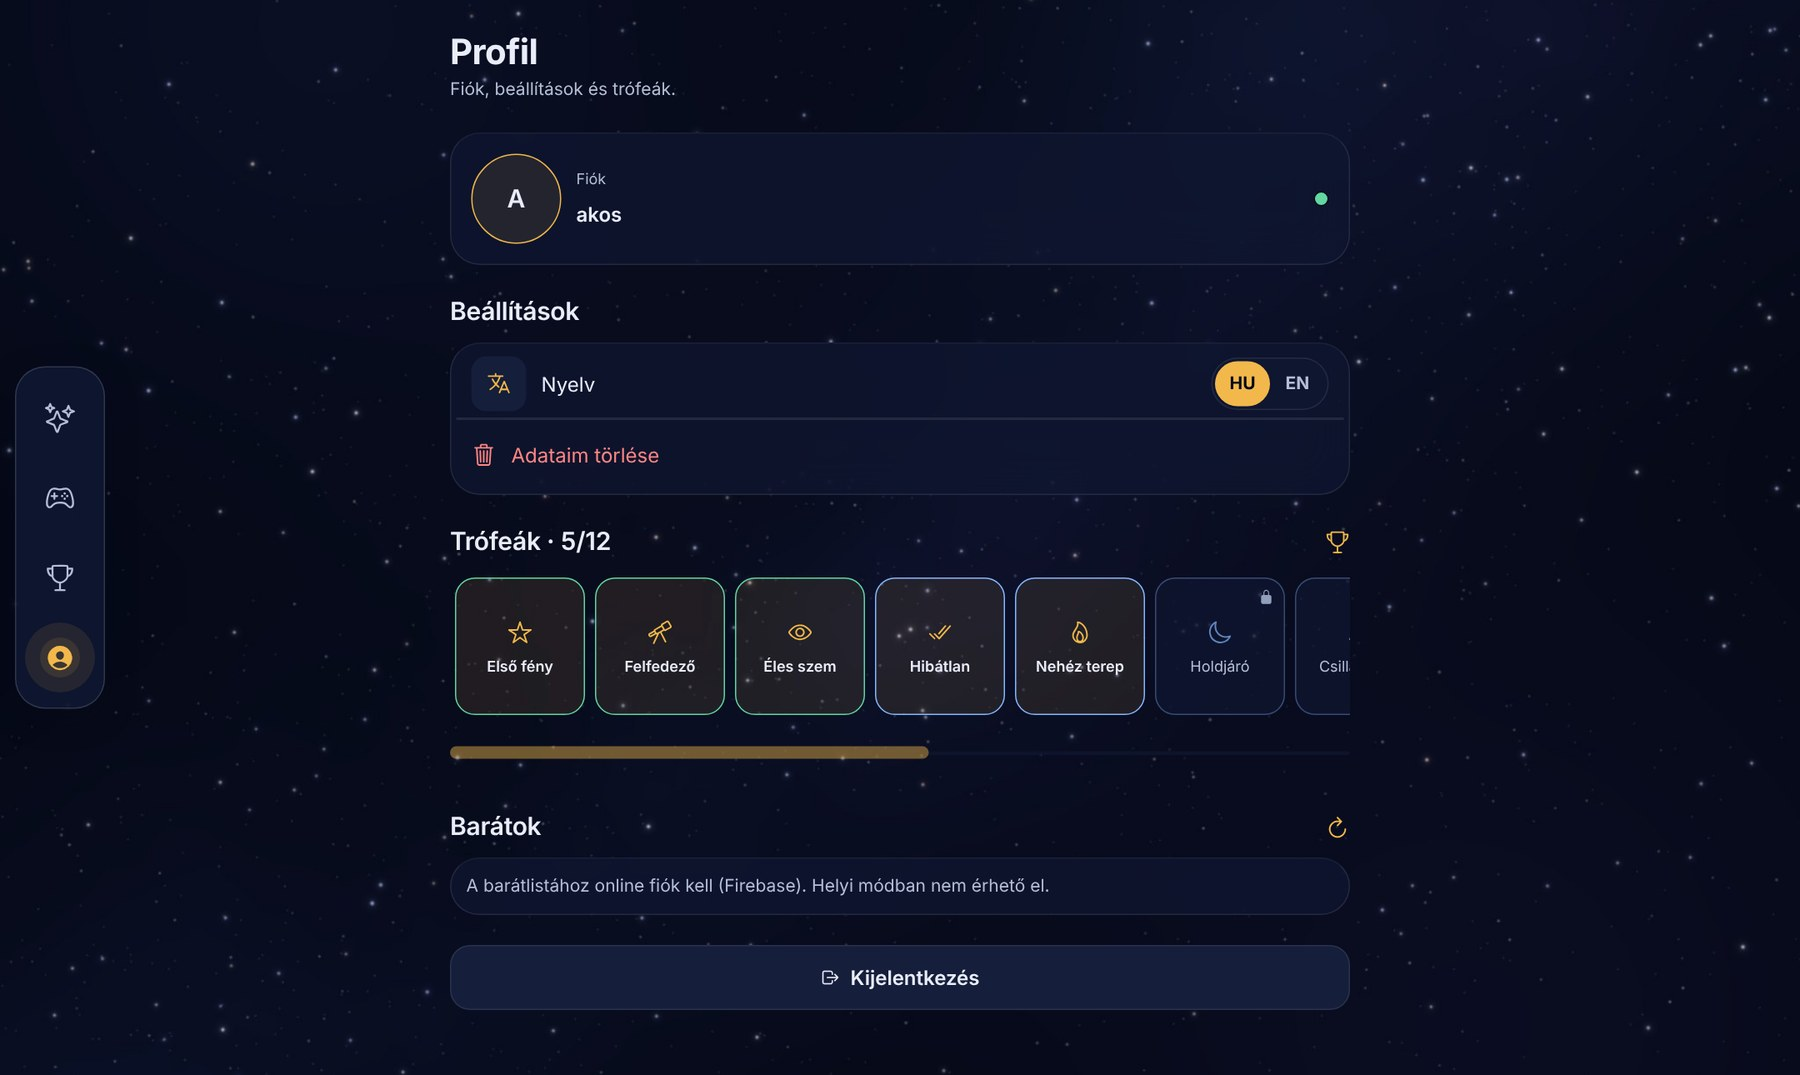
\includegraphics[width=0.82\linewidth]{kepek/profil.jpg}
  \caption{A profil képernyő}
  \label{fig:profil}
\end{figure}

\textbf{Profil:} itt látható a fiók neve, itt váltható a nyelv, itt kérhető az adatok törlése, és
itt követhetők a trófeák (megszerzett és zárolt állapotban, \kod{x/12} számlálóval), valamint a
barátlista (\ref{fig:profil}.~ábra). Helyi módban a barátlista nem érhető el, mert ahhoz online
fiók szükséges.

\begin{figure}[H]
  \centering
  \begin{subfigure}[t]{0.32\linewidth}
    \centering
    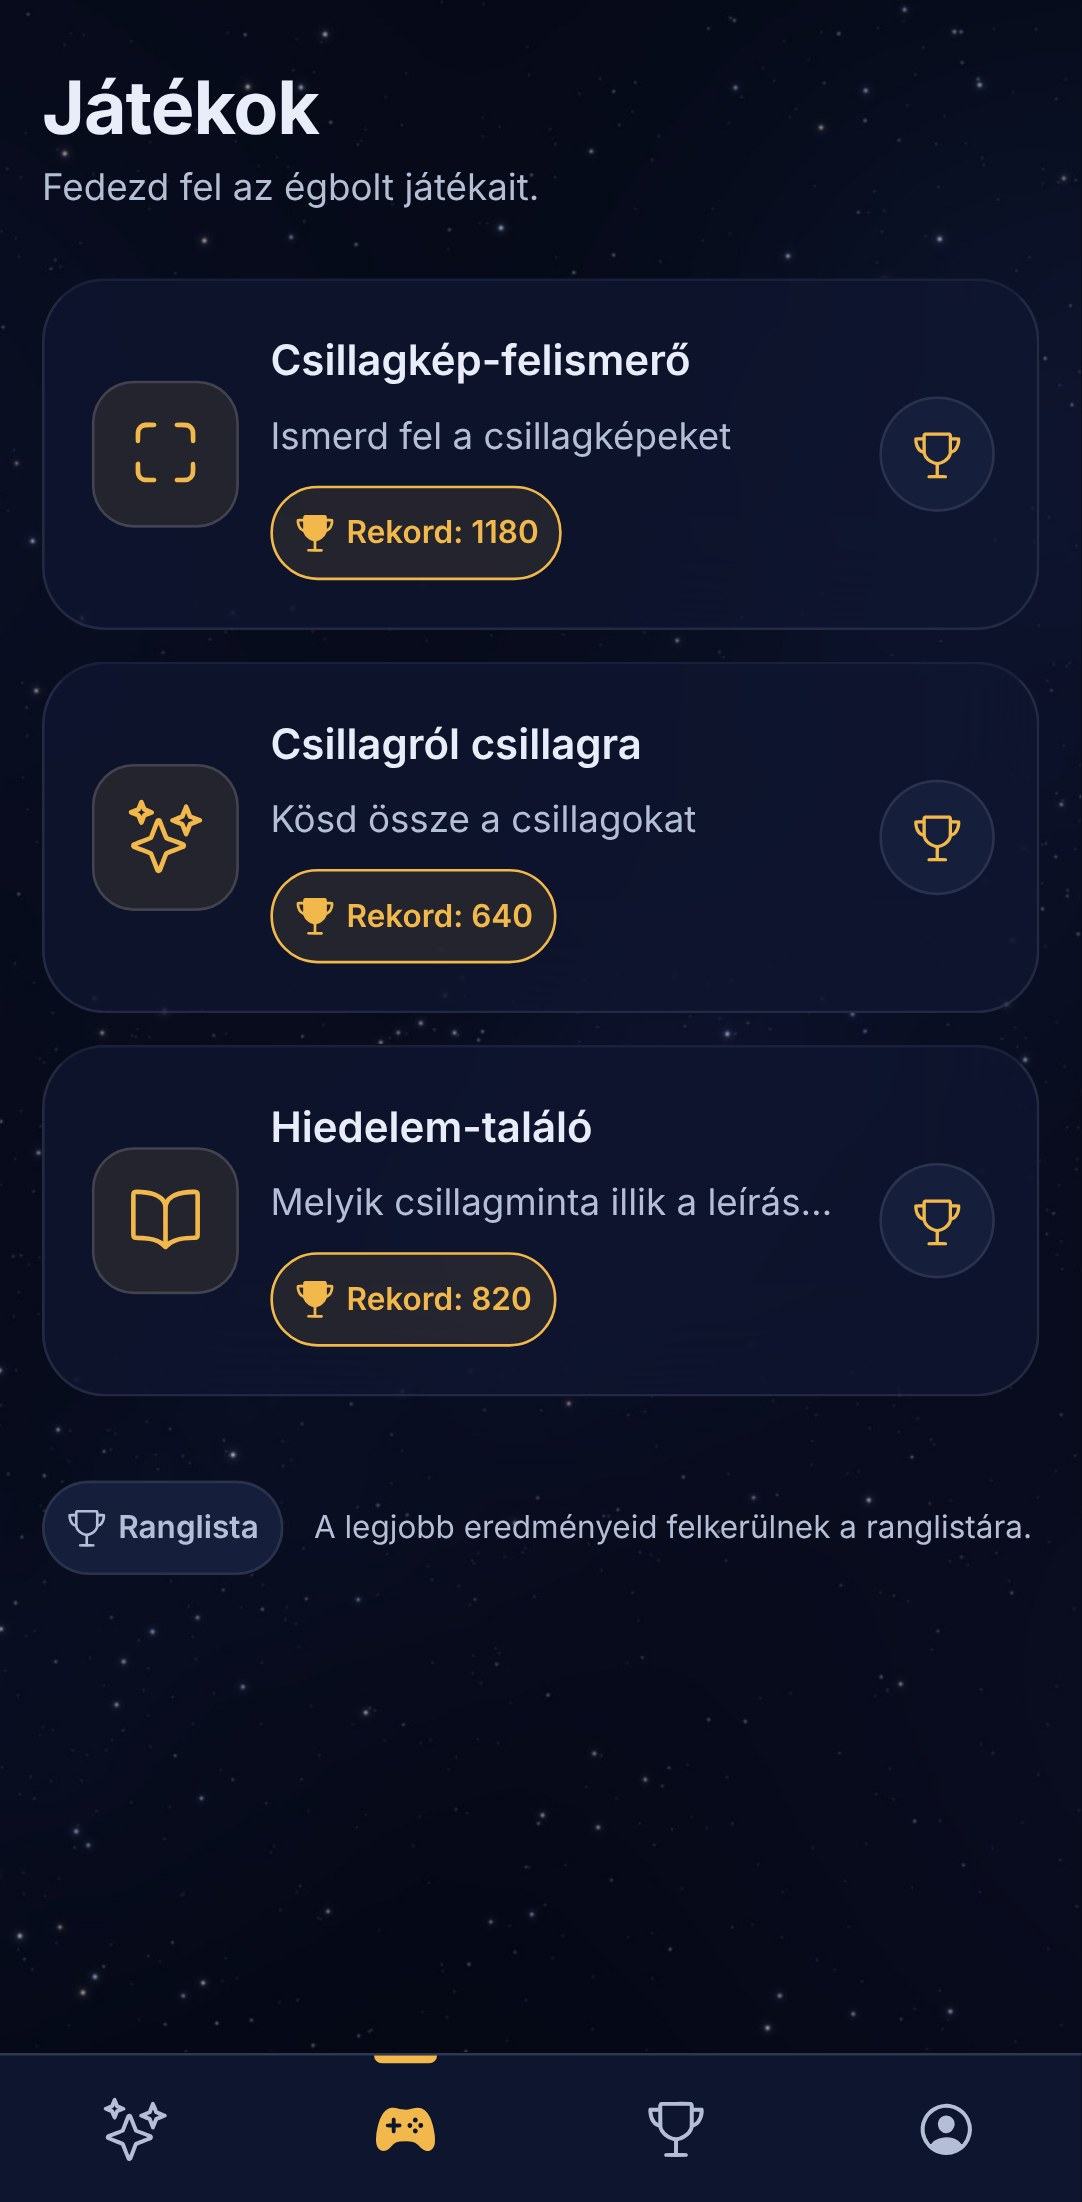
\includegraphics[width=\linewidth]{kepek/telefon-jatekok.jpg}
    \caption{Játékok}
  \end{subfigure}\hspace{1cm}
  \begin{subfigure}[t]{0.32\linewidth}
    \centering
    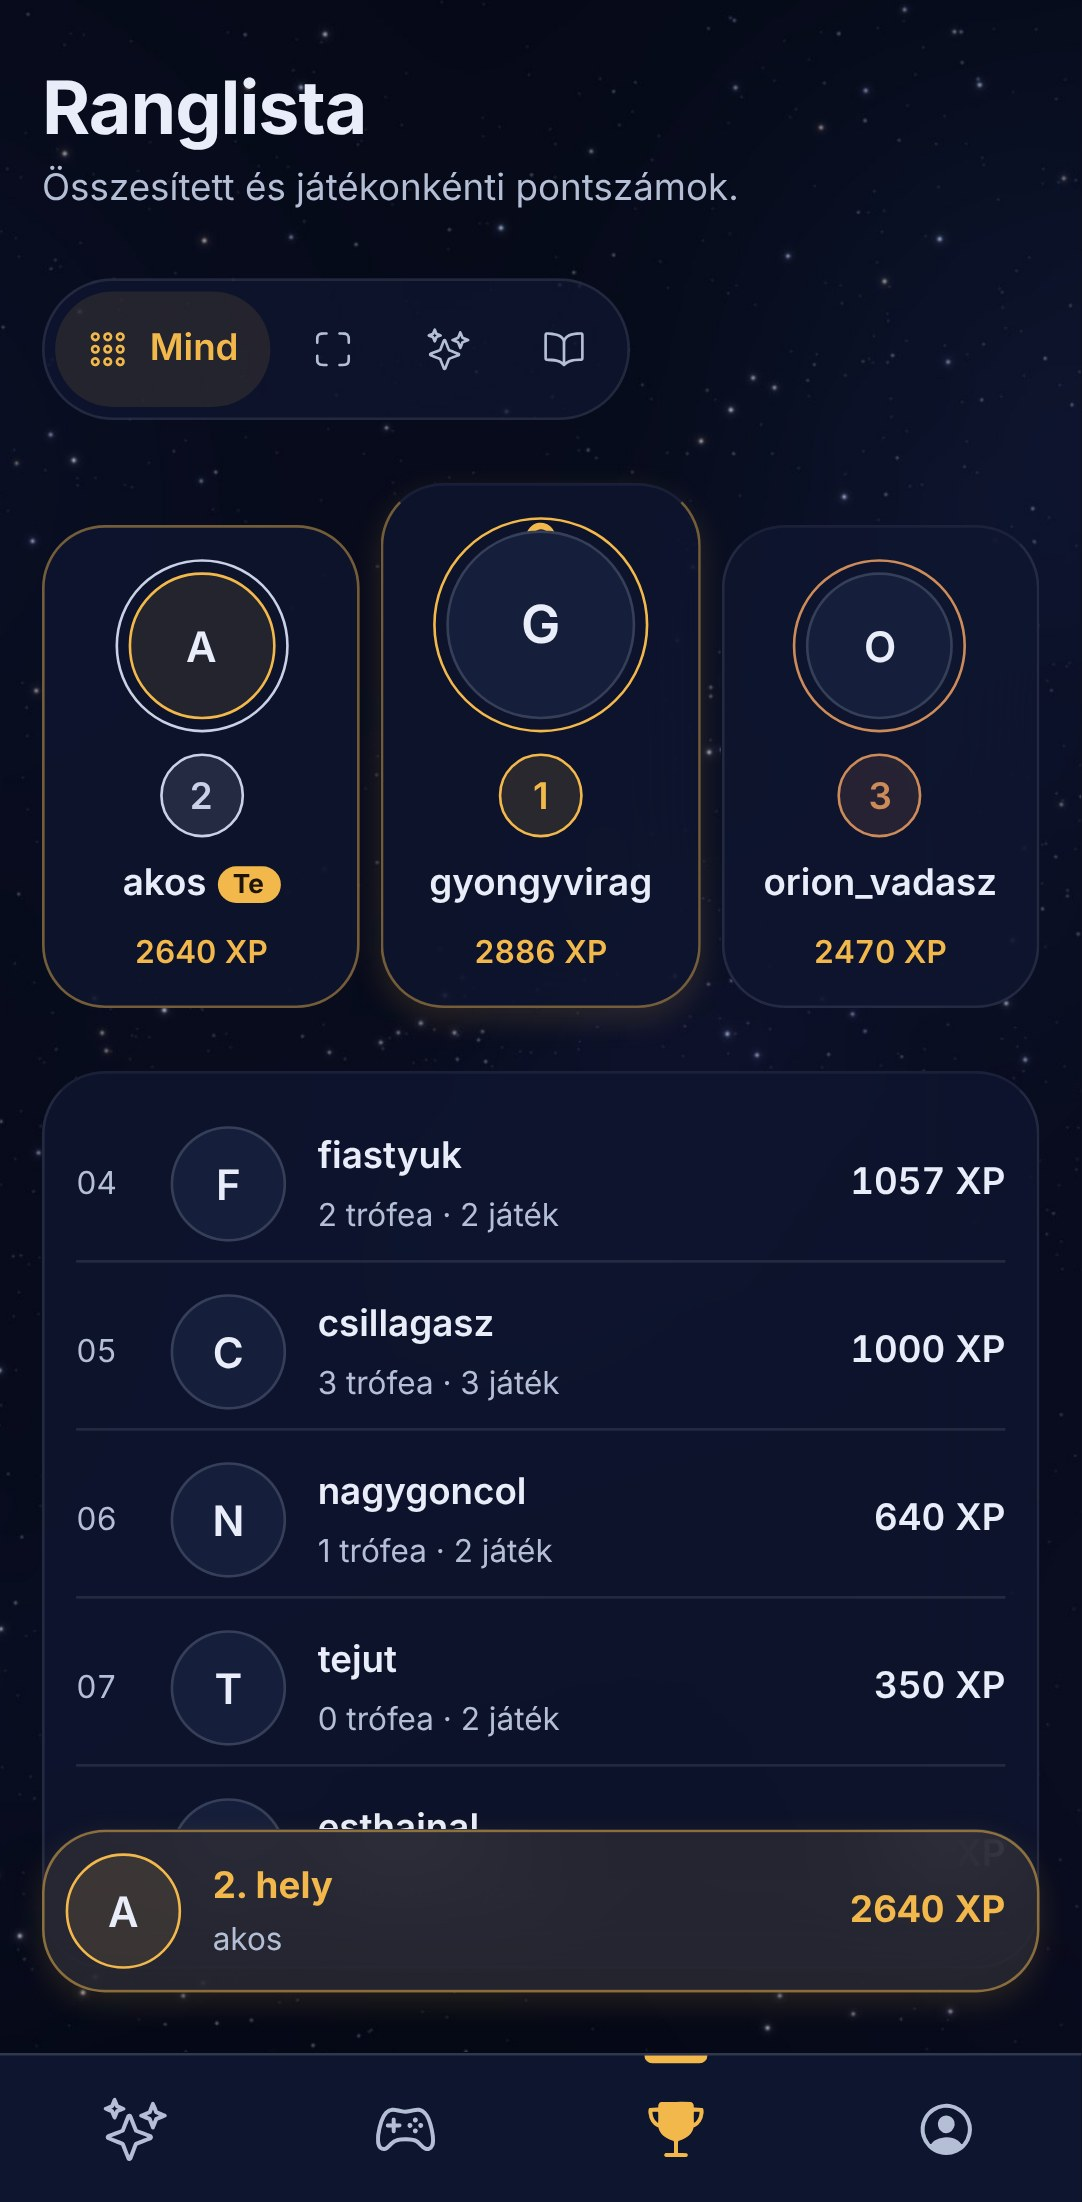
\includegraphics[width=\linewidth]{kepek/telefon-ranglista.jpg}
    \caption{Ranglista}
  \end{subfigure}
  \caption{Telefonos nézet: alsó ikonsáv, ujjal lapozható oldalak}
  \label{fig:telefon}
\end{figure}

\textbf{Telefonos elrendezés:} kis képernyőn a menü az alsó, teljes szélességű ikonsávba kerül
(\ref{fig:telefon}.~ábra). Az oldalak között vízszintes húzással is lehet lapozni: a
szomszédos oldal az ujjal együtt csúszik be, az aktív oldalt jelző arany vonal pedig követi a
mozdulatot.

% A képernyőképek mind a saját alfejezetükben jelenjenek meg, a Hardver előtt
\FloatBarrier
\subsection{Hardver}

Mivel az alkalmazás a csillagokat egyetlen rajzolási hívással jeleníti meg, és a jelenetet
csak változáskor rajzolja újra, a gépigénye alacsony: a legtöbb mai számítógépen és okostelefonon
gördülékenyen fut.

\subsubsection*{Minimális rendszerkövetelmények}

\begin{itemize}
  \item \textbf{Webes változat:} WebGL-t támogató, friss böngésző (Chrome, Edge, Firefox vagy
        Safari), integrált videókártya is elegendő.
  \item \textbf{Android:} Android 7.0 vagy újabb (az Expo SDK 58 követelménye).
  \item \textbf{iOS:} iOS 16.4 vagy újabb (az Expo SDK 58 követelménye).
  \item \textbf{Memória:} 2 GB RAM ajánlott; az adatok (csillagkatalógus, kultúrák) mérete
        néhány megabájt.
  \item \textbf{Hálózat:} az égbolt böngészéséhez nem szükséges; a fiókhoz, a ranglistához és a
        barátlistához internetkapcsolat kell.
  \item \textbf{Helymeghatározás (opcionális):} GPS vagy a böngésző helymeghatározása; enélkül
        egy előre megadott város választható.
  \item \textbf{Beviteli eszközök:} érintőképernyő, vagy egér és billentyűzet.
\end{itemize}

\subsubsection*{Fejlesztői környezet}

A fejlesztéshez Node.js 22 (LTS) és npm szükséges; az adatszkriptekhez Python 3, a Firebase
emulátoros integrációs tesztekhez Java. Az alkalmazás az \kod{npm install} és az \kod{npm start}
parancsokkal indul, a webes változat az \kod{npm run web} paranccsal.

\subsection{Tesztelés és kódminőség}

A logikai réteg függvényeit 36 tesztfájlban összesen 361 egységteszt ellenőrzi (Jest), többek
között a csillagászati számításokat, a játékok pontozását és a kérdések összeállítását, a
trófeák feltételeit, a ranglista rangsorolását, a fordítások teljességét és a naplózás
adattisztítását. A Firebase-hitelesítést külön integrációs tesztek ellenőrzik a helyi Firebase
emulátorral. A kód minőségét a TypeScript típusellenőrzése (\kod{npm run typecheck}), az ESLint
(\kod{npm run lint}) és a Prettier (\kod{npm run format:check}) biztosítja.

% =====================================================================
\section{Összegzés}

A projekt során sikeresen elkészült egy webes és mobilos csillagnéző alkalmazás, amely
valós időben, csillagászatilag pontosan mutatja az eget bármely helyről és időpontból, és 18 égi
kultúra - köztük a magyar népi égbolt - csillagképeit és legendáit teszi elérhetővé, magyarul
és angolul. A három játék, a trófeák, az online ranglista és a barátlista a böngészést játékos
tanulással és versenyhelyzettel egészíti ki. A háromrétegű felépítés és a cserélhető
(Firebase-es vagy helyi) szolgáltatások miatt az alkalmazás Firebase nélkül is bemutatható és
fejleszthető. A kitűzött funkcionális követelmények teljesültek, a kódot automatikus tesztek és
statikus ellenőrzések védik.

\subsection{További fejlesztési lehetőségek}

Az alkalmazás jelenlegi változata stabil alapot biztosít, de számos irányban továbbfejleszthető:

\textbf{Tájpanoráma a horizonton:} a Stellariumhoz hasonlóan dombok, fák, épületek sziluettje a
horizont mentén, amely viszonyítási alapot ad; a táj mögé eső csillagképek nevei el is
rejthetők.

\textbf{Kiterjesztett valóság (AR) mód:} a projekt eredeti ötlete egy kameraképre vetített
égbolt volt; a telefon iránytűje és gyorsulásmérője alapján a nézet követhetné a készülék
irányát.

\textbf{Naprendszer-égitestek:} a Nap, a Hold és a bolygók megjelenítése, valamint nappali égbolt
és szürkület.

\textbf{Csillagok sajátmozgása:} jelenleg a precesszió módosítja a csillagok helyét; a
sajátmozgás figyelembevételével az évezredes időutazás még pontosabb lenne.

\textbf{Szerveroldali eredmény-ellenőrzés:} a pontszámokat jelenleg a kliens számolja;
felhőfüggvényekkel (Cloud Functions) a ranglista csalásbiztossá tehető.

\textbf{További tartalom és nyelvek:} újabb égi kultúrák és leírások, a magyar népi
égbolt bővítése, újabb felületi nyelvek; mindehhez a jelenlegi adatformátum már alkalmas.

\textbf{Közzététel:} a webes változat publikálása (például Firebase Hostingon), valamint Android-
és iOS-telepítőcsomag készítése az Expo felhőalapú buildszolgáltatásával (EAS Build).

\end{document}
